\documentclass[journal=jpcbfk,manuscript=article]{achemso}

\usepackage{graphicx}
\usepackage{wrapfig}
\usepackage{subcaption}
\usepackage{amsmath} % or simply amstext
\usepackage{amssymb}
\usepackage{siunitx}
\usepackage{booktabs}
\usepackage[export]{adjustbox}
\newcommand{\angstrom}{\textup{\AA}}
\usepackage{cleveref}
\usepackage{booktabs}
\usepackage{gensymb}
\usepackage{float}
\usepackage{xr}
\usepackage{enumitem}
\newcommand{\nclusters}{10}
%\DeclareUnicodeCharacter{03C9}{$\omega$}
\externaldocument[S-]{Supporting_Information}

\SectionNumbersOn

\title{Statistical Inference of Transport Mechanisms and Long Time Scale Behavior from Time Series 
       of Solute Trajectories in Nanostructured Membranes}
\author{Benjamin J. Coscia}
\affiliation{Department of Chemical and Biological Engineering, University of Colorado Boulder, Boulder, CO 80309, USA}
\author{Christopher P. Calderon}
\affiliation{Department of Chemical and Biological Engineering, University of Colorado Boulder, Boulder, CO 80309, USA}
\author{Michael R. Shirts}
\email{michael.shirts@colorado.edu}
\affiliation{Department of Chemical and Biological Engineering, University of Colorado Boulder, Boulder, CO 80309, USA}

\begin{document}

  \graphicspath{{./figures/}}
  \maketitle
  
  \begin{abstract}

  Appropriate time series modeling of complex diffusion in soft matter systems on the
  microsecond time scale can provide a path towards inferring transport mechanisms and
  predicting bulk properties characteristic of much longer time scales. In this work 
  we apply the sticky hierarchical Dirichlet process hidden Markov model (HPD-AR-HMM) 
  %MRS: might be confusing to have the AR in there when the words ``Auto-regressive'' 
  %don't appear; then they would try to figure out where the AR is. 
  to solute center-of-mass trajectories generated from long molecular dynamics 
  simulations in a cross-linked inverted hexagonal phase lyotropic liquid crystal
  (LLC) membrane in order to automatically detect a variety of solute dynamical states
  which can be further explained in terms of solute-membrane interactions.

  We group the states identified by the HDP-AR-HMM into clusters based on multiple metrics
  aimed at distinguishing solute behavior based on their fluctuations, dwell times
  in each state and position within the inhomogeneous membrane structure. We analyze
  prevalent clusters in order to relate their parameters to physical interactions between 
  solutes and the membrane. 
  Along with parameters of individual states, the HDP-AR-HMM simultaneously infers a transition
  matrix which allows us to stochastically propagate solute behavior from all of the 
  independent trajectories onto much longer time scales while still preserving the 
  qualitative behavior characteristic of the MD trajectories. This affords a direct 
  connection to important macroscopic observables used to characterize performance like
  solute flux and selectivity. 

  %MRS: we have to decide if ``effective'' is the right word. Alternative is ``promising''.
  Overall, this work provides an effective way to simultaneously identify transport 
  mechanisms in nanoporous materials and project complex diffusive behavior on
  long time scales.  
  %MRS: simplify by removing nominalizations.
  %This enhancement to our understanding 
  Our enhanced understanding
  of the diverse range 
  of solute behavior allows us to hypothesize design changes 
  to LLC monomers aimed towards controlling the rates of solute passage, thus improving 
  the selective performance of LLC membranes. 
  
  \end{abstract}  
  
  \section{Introduction}
  
  There is a need for highly selective membranes in order to perform efficient 
  separations of the components of complex aqueous streams. Seawater and
  brackish water desalination, separation of organic micropollutants from 
  municipal water supplies, recovering valuable dissolved species from 
  waste stream and creating breathable barriers to harmful contaminants are just a
  subset of the broad range of applications for selective membrane separations.~\cite{fritzmann_state---art_2007,fonseca_couto_critical_2018,dischinger_evaluation_2019,ramaseshan_functionalized_2006}
  While researchers often focus on membrane permeability, many argue that
  it may be more beneficial to focus on membrane selectivity in order to 
  reduce the costs of commercial nanofiltration and reverse osmosis.~\cite{werber_materials_2016}
  
  The ability to efficiently design novel membrane materials for selective separations
  would be greatly enhanced by easily interpretable methods for connecting microscopic
  fluctuations with macroscopic observables. If one could apply molecular dynamics 
  (MD) simulations to explain important experimental metrics such as solute flux and 
  selectivity in terms of detailed chemically dependent solute motion, then we can more
  easily bridge the disconnect between theory and application. In many systems, it is 
  possible to achieve this by calculating diffusion constants. 
  % BJC4: even if we could calculate diffusion constants, wouldn't there still be value 
  % in understanding chemical detail?
  % BJC4: It might not be a good idea to blame our need for this modeling on non-linear MSDs, 
  % especially since our MSDs appear to be at or nearing a linear regime.
  % BJC4: seems like we should be addressing the problem as short time scale subdiffusive 
  % dynamics that dictates measurable long time scale diffusion. Although curves become linear,
  % the slopes should be a product of the short time scale motion.
  Unfortunately, for 
  systems which exhibit complex short timescale subdiffusive dynamics, one cannot 
  reliably compute diffusion constants since solute mean square 
  displacements (MSDs) are non-linear on the timescales accessible to molecular simulation.
  Therefore, we are in need of a more flexible approach for modeling solute dynamics
  which makes less assumptions about the solute's short time scale behavior.
  
  In this work, we are particularly interested in the design of lyotropic liquid 
  crystal (LLC) monomers, a class of amphiphilic molecules whose ordered self-assembled
  phases can be cross-linked into mechanically strong membranes capable of highly 
  selective separations. Inverted hexagonal, H\textsubscript{II}, phase LLC membranes
  are characterized	by hexagonally packed, uniform-sized and straight pores, an ideal
  geometry for high throughput transport. Their pores are lined with the LLC monomer's
  functional groups which can potentially be designed to interact with solutes in a 
  chemically-specific manner. It would be extremely useful to experimentalists if we 
  could connect LLC monomer design with measurable quantities. This goal is complicated
  by the non-Brownian hopping and trapping behavior induced by the membrane's diverse
  topology and inhomogeneous structure result in subdiffusive behaviour out to multiple microseconds of simulation.~\cite{coscia_understanding_2019,coscia_chemically_2019}
  %MRS: to sentence above added to come back to main theme

  We have already advanced our understanding of LLC monomer design in our previous work
  by building stochastic time series models based on the chemical intuition gained
  from qualitative MD studies of solute transport in an H\textsubscript{II} phase LLC
  membrane.~\cite{coscia_chemically_2019,coscia_capturing_2020} We identified three 
  classes of trapping behavior which result in 
  %MRS: tweaked
  subdiffusion out to the microsecond time scale. 
  In our 
  first approach to stochastically model this behavior, we treated the system's dynamics
  as a sequence of anti-correlated hops between power law distributed periods of 
  entrapment, a framework called subordinated fractional Brownian or L\'evy
  motion.~\cite{thiel_weak_2014,teuerle_modeling_2013} In a second approach, we treated 
  solute motion as a Markov state model~\cite{pande_everything_2010} with state-dependent
  dynamics, where we parameterized the state transition probabilities between each of
  eight discrete states, defined by the observed trapping mechanisms, as well as the 
  solute dynamics within each of these states. We showed how one could use realizations
  of any stochastic model like these in order to predict macroscopic flux and selectivity. 
  
  Although powerful and insightful, our previous work required considerable human effort
  in order to analyze the MD trajectories and to hypothesize stochastic models which
  matched the behavior of solutes. It would be significantly more useful and broadly 
  applicable if we could design an approach which 
  %MRS: tweaked to sound more machine-learning-y
  %automatically 
  distinguishes and 
  parameterizes varied solute dynamics 
  in a data-driven way
  and leaves a facile way to generate an ensemble
  of stochastic trajectory realizations that can be used to predict macroscopic transport
  properties.
  
  In this work we attempt to minimize human effort through a novel application of 
  the sticky hierarchical Dirichlet process autoregressive hidden Markov model 
  (HDP-AR-HMM), a nonparameteric Bayesian classification technique that allows the user to 
  automatically detect and infer the parameters of an unknown number of latent vector
  autoregressive (VAR) modes present in solute center-of-mass MD 
  trajectory.~\cite{fox_bayesian_2010} The sticky HDP-AR-HMM greatly extends the 
  basic framework of simpler but more limited finite hidden Markov modeling approaches.
    
  In their most basic form, hidden Markov models (HMMs) are used to generate
  a series of latent, or hidden, states dependent only on the previous state.~\cite{rabiner_tutorial_1989}
  Propagating an HMM generates sequential but independent observations from 
  the emission distributions associated with each hidden state. Transitions 
  between states are mathematically defined by a matrix of transition probabilities.
  Given a series of observations and a known number of hidden states, the 
  Baum-Welch algorithm is the most commonly used way to determine the hidden
  state sequence and the underlying parameters of a standard HMM.~\cite{baum_maximization_1970}
  It also possible to achieve the same results using a Bayesian 
  framework.~\cite{scott_bayesian_2002,jasra_markov_2005} 
  %MRS: not entirely clear what purpose of above sentence its - it sort of implied you will use Bayesian framework?
  One can place priors
  on the transition probabilities and parameters of the hidden states' emission
  distributions in order to iteratively infer their values and to estimate the hidden state
  sequence. 
  HMMs have been used in a broad range of applications including speech
  recognition, weather forecasting and bioinformatics.~\cite{juang_hidden_1984,hughes_non-homogeneous_1999,yoon_hidden_2009}.
  In molecular simulations, HMMs have been
  used to characterize molecular kinetics in order to determine the equilibrium 
  distribution of various observables.~\cite{noe_probability_2008}
  %MRS: probably a few more citations that should be added above, since there has been a lot.
  By placing a hierarchical Dirichlet process (HDP) prior on the transition 
  probabilities, it is possible to extend HMMs to an unknown number of hidden
  states, thus allowing the model's complexity to be driven by the complexity
  of the data.~\cite{teh_hierarchical_2006} We will refer to this as the HDP-HMM,
  although in literature it is often called the infinite hidden Markov 
  model.~\cite{beal_infinite_2002} The HDP-HMM elegantly overcomes the main
  shortcoming of standard HMMs, the need to choose the number of states 
  \textit{a priori}, making its use more advantageous in a diversity of 
  applications including economic data and single particle trajectory 
  analysis.~\cite{shi_identifying_2016,hines_analyzing_2015} 

  One issue with the original formulation of the HDP-HMM is that it does 
  not distinguish self-transitions and transitions between different states.
  Practically, this can result in rapid switching between states and inferred
  state sequence representations that do a poor job of describing the 
  observations. Fox et al. addressed this issue by adding a `sticky' 
  parameter.~\cite{fox_sticky_2007} The sticky HDP-HMM is useful in situations
  where the user has prior knowledge that state persistence is likely.
  For example, in the case of speaker diarization, it is unlikely that a 
  conversation between two people would rapidly switch between speakers.~\cite{fox_sticky_2011}
  This is also important for our work where we expect state persistence due
  to solute entrapment.   
  
  The usefulness of the sticky HDP-HMM has been further extended to include 
  temporal dependencies common to many real datasets. State dynamics and 
  relaxation into new states are often correlated.~\cite{calderon_data-driven_2014}
  Fox et al. formulated a method that accounts for this behavior by
  incorporating Markov jump linear systems (MJLSs) into infinite state 
  models.~\cite{fox_nonparametric_2009} An MJLS models each dynamical mode
  as a linear dynamical process. Two MJLS sub-classes are switching linear
  dynamical systems (SLDSs) and switching vector autoregressive (VAR) processes.
  Switching VAR processes are similar to SLDSs except that they do not
  incorporate measurement noise. Since MD simulations do not contain measurement
  noise, we will model the dynamical modes exhibited by MD solute trajectories 
  as VAR processes and we will refer to our model as an application of the 
  sticky HDP-AR-HMM in order to maintaining its distinction from the even more
  general sticky HDP-SLDS models.
  
  %MRS: define what ``this'' is - important claim, make it clear what it is you are claiming.
  To our knowledge, this is a novel application and analysis of the sticky 
  HDP-AR-HMM. Typical applications center around determining the number of
  states, the state sequence and occasional analysis of the emission 
  distributions. The addition of temporal correlation to the inference 
  procedure has primarily been used to improve state sequence 
  identification.~\cite{calderon_inferring_2015,hamada_modeling_2016}
  Not only do we use the HDP-AR-HMM to segment MD time series into distinct
  dynamical modes, but we cluster and analyze the temporally-correlated 
  parameters of the model in order to learn physical mechanisms and describe
  solute kinetics. Further, we use the model parameters to generate new 
  time series trajectories which enable projections of MD simulations on 
  much longer time scales.
  
  %BJC4: enumerate?
  %BJC4: might be able to condense this since some of it repeats above.
  We aim to address two primary scientific questions with this work:
  First, we want to know whether it is possible to use the HDP-AR-HMM to 
  help us predict macroscopic transport properties. We use the VAR parameters
  and state transition probability matrix of the HDP-AR-HMM in order to 
  generate stochastic trajectory realizations with behavior similar to that
  exhibited by MD. One can project these realizations onto much longer 
  timescales with computational ease extending into timescales where 
  regular diffusive behavior again occurs.
  Second, we want to know if the HDP-AR-HMM algorithm can help researchers
  efficiently uncover underlying transport mechanisms which give rise to different 
  solute dynamical behavior.
  We use the parameters of the states identified by the HDP-AR-HMM in order to infer 
  dominant solute-membrane interactions and transport mechanisms. We cluster similar 
  state parameters in order to reduce the state space and to understand which segments 
  of the solute trajectories exhibit similar behavior. We support our mechanistic 
  hypotheses via quantitative comparison to various physical membrane properties and
  solute-membrane interactions.
  
  \section{Methods}
    
  We ran all MD simulations and energy minimizations using GROMACS 2018.~\cite{bekker_gromacs:_1993,berendsen_gromacs:_1995,van_der_spoel_gromacs:_2005,hess_gromacs_2008}  
  Our Python implementation of the HDP-AR-HMM algorithm is available online at \\
  %MRS: possibly should give the permanent reference to a shirtsgroup fork?  We can discuss which is likely to be more permenant
  \texttt{https://github.com/bencoscia/hdphmm}. All other post-simulation 
  trajectory analysis tools are available online at
  \texttt{https://github.com/shirtsgroup/LLC\_Membranes}.

  \subsection{Molecular Dynamics Simulations}

  We studied transport of solutes in the H\textsubscript{II} phase using an
  atomistic molecular model of four pores in a monoclinic unit cell with 
  10\% water by weight. Approximately one third of the water molecules 
  occupy the tail region with the rest near the pore center.%MRS: cite previous paper here on this.
  
  We chose to study a subset of 4 of the fastest moving solutes from our previous
  work: methanol, acetic acid, urea and ethylene glycol.
  In addition to exploring membrane structural space the most, these solutes have a
  relatively diverse set of chemical functionality. For each solute we created a 
  separate system and to each system we added 6 solutes per pore for a total of 24 solutes. This number 
  of solutes per pore provides a balance of a low degree of interaction between 
  solutes and a sufficient amount of data from which to generate statistics on the
  time scales which we simulate. Further details on the setup and equilibration of
  these systems are detailed in our previous work.\cite{coscia_chemically_2019}
  
  %MRS: tweaked
  %We let each solute undergo 
  Each solute system was simulated for 5 $\mu$s of molecular dynamics  simulation. We used a time step of 2 fs
  at a pressure of 1 bar and temperature of 300K controlled by the Parrinello-Rahman 
  %MRS: just wondering, was this semiisotropic, or isotropic?  If isotropic, do we know how different the diagonals of the 
  pressure tensor were (since the system is not totally isotropic)
  barostat~\cite{parrinello_polymorphic_1981} and velocity rescale 
  thermostat~\cite{bussi_canonical_2007} respectively. We recorded configurations every 0.5 ns.

  \subsection{Applying the sticky HDP-AR-HMM to MD Trajectories}\label{method:HDP-AR-HMM}

  % BJC4: Chris' general comment for this section: 'the problem with this section is 
  % that it doesn't help the expert or novice figure out what is being done (either 
  % expand more or relegate details to references and talk bigger picture)'
  
  % BJC4: I think it makes sense to stick to bigger picture since there are much
  % better descriptions in literature. I haven't made any modifications to what's already been done
  
  % BJC4: replaced with what follows. Lots of the big picture is in the intro
  
%  \subsubsection*{Extending Hidden Markov Modeling to an Unknown Number of States}
%  
%  Hidden Markov models (HMMs) are a useful and widely used technique for modeling
%  sequences of observations where the probability of the next observation in a 
%  sequence depends, at least in part, on a previous unobserved, latent or hidden,
%  state.~\cite{beal_infinite_2002} In the context of our simulations, the observations
%  correspond to the center of mass coordinates of the solutes versus time, and the
%  states correspond to segments of the trajectory with similar dynamical behavior 
%  which gives rise to those types of observations. The probability of transitioning 
%  to a state based on the current state is defined in terms of an $n\times n$ 
%  transition probability matrix, $T$, where $n$ is the number of states. Unfortunately,
%  standard HMMs require $n$ to be known \textit{a priori}. One can partially overcome
%  this by testing a range of numbers of hidden states and determining which is the
%  best representation of the data.~\cite{pohle_selecting_2017}
%  
%  The infinite-state HMM overcomes this drawback by placing a hierarchical
%  Dirichlet process (HDP) prior on the transition probabilities.~\cite{fox_bayesian_2010} Using some 
%  base probability distribution, $H$, a Dirichlet process (DP) generates discrete 
%  distributions, $G_0$, over a countably infinite number of probability measures:
%  \begin{equation}
%      G_0 = \sum_{k=1}^{\infty} \beta_k \delta_{\theta_k} ~~ \theta_k \sim H, \beta \sim GEM(\gamma)
%  \end{equation}
%  where the $\theta_k$ are values drawn from the base distribution and the weights
%  $\beta_k$ come from a stick-breaking process parameterized by the concentration 
%  parameter $\gamma$ (equivalently referred to as GEM($\gamma$)).~\cite{halmos_random_1944} In shorthand, this
%  specification can be expressed as $G_0 \sim DP(\gamma, H)$. The concentration 
%  parameter, $\gamma$, expresses one's confidence in the base distribution $H$.
%  We use a uniform base distribution for $H$. When $\gamma\to 0$, the first 
%  weight of $G_0$, $\beta_1$, approaches unity and for $\gamma\to\infty$, the weights
%  become uniform and $G_0$ closely resembles $H$. Each row, $G_j$, of the transition 
%  matrix is produced by drawing from a DP specified using the $\beta$ vector as a 
%  discrete base distribution and a separate concentration parameter, $\alpha$.
%  \begin{equation}
%      G_j = \sum_{k=1}^{\infty} \pi_{jk} \delta_{\theta_k} ~~ \pi_j \sim DP(\alpha, \beta)
%  \end{equation}
%  This hierarchical specification ensures that the transition probabilities in 
%  each row share the same support points \{$\theta_1$, ..., $\theta_k$\}.
%  Once the model has converged only a finite number of states will have significant
%  sampling.

  We use the sticky HDP-AR-HMM in order to assign the time-correlated positional 
  fluctuations of solute center-of-mass MD trajectories to discrete dynamical modes while 
  simultaneously inferring the VAR parameters of those modes. We use the sticky model
  in order to emphasize self-transitions since we expect solutes to stay trapped in
  states for appreciable amounts of time. We analyze solute motion in terms of their
  cylindrical coordinates, $(r, z)$, with the $z$ axis oriented along the membrane 
  pores and the radial dimension, $r$, measured from the closest pore center. 
  
  Although the discussion will be presented in terms of 2D cylindrical coordinates, we
  applied the HDP-AR-HMM algorithm to 3D solute center-of-mass coordinate trajectories 
  with the radial dimension represented by the solute's $x$ and $y$ coordinates 
  transformed relative to the nearest pore center. By working in Cartesian coordinates,
  we avoid mathematical complexity introduced by change of coordinates into cylindrical
  coordinates while estimating the state sequence.

  %MRS: some of this is a repetition of what you said above.
  We implemented the sticky HDP-AR-HMM in Python 
  (\texttt{https://github.com/bencoscia/hdphmm}) which we heavily adapted from
  the MATLAB code of Fox et al.~\cite{fox_nonparametric_2009} Since we do not incorporate
  any novel methodology to the HDP-AR-HMM inference procedure, we refer the 
  interested reader to an excellent and in-depth description of the formulation of
  the HDP-AR-HMM and related models.~\cite{fox_bayesian_2010}
  
  %\subsubsection*{Parameterizing the Hidden States}\label{method:var_params}
  \textit{Parameterizing the Hidden States}: We describe the dynamics of each 
  state visited by solutes in our MD simulations using a first order vector 
  autoregressive (VAR(1)) model. In general, a VAR($r$) process is characterized by a
  vector of observations in a time series that are linearly dependent on $r$ previous
  values of the time series vector:
  \begin{equation}
  	\mathbf{y}_t = \mathbf{c} + \sum_{i=1}^r A_i\mathbf{y}_{t-i} + \mathbf{e}_t~~~~\mathbf{e}_t \sim \mathcal{N}(0, \Sigma)
  \label{eqn:var}
  \end{equation}
  Previous observations are weighted by coefficient matrices, $A_i$. The VAR($r$) 
  process is further characterized by a shift in the mean of each dimension by the
  vector $\mathbf{c}$ and a white noise term $\mathbf{e}_t$.~\cite{hamilton_time_1994}
  We assumed $\mathbf{e}_t$ to be multivariate Gaussian noise, with mean zero and
  covariance, $\Sigma$. We limited our analysis to an autoregressive order of $r=1$.
  This means that we only parameterize $A_1$. To simplify notation, we will call it $A$. 
  We used a conjugate matrix-normal inverse-Wishart (MNIW) prior on parameters 
  $A$ and $\Sigma$ and a Gaussian prior on $\mathbf{c}$ in order to infer their 
  values.~\cite{fox_nonparametric_2009}
   
%  \subsubsection*{Applying the HDP-AR-HMM to MD Trajectories} 
  
  \textit{State sequence and parameter inference}: We inferred the 
  state sequence and parameters for each of the 24 solute trajectories independently.
  Although the HDP-AR-HMM is capable of identifying an infinite number of states, 
  a Dirichlet process tends to exhibit a ``rich get richer" effect, favoring
  a fewer number of states.~\cite{dreyer_discovering_2011} By applying the algorithm to each trajectory 
  independently, we reduce the possibility of lumping together multiple 
  similar states which we would prefer to stay separated before clustering.
  
  We ran 2000 iterations of the HDP-AR-HMM procedure on each trajectory which
  was sufficient in order to arrive at converged state sequences and VAR parameter
  estimates. By our criteria, the procedure generally converged within 500--1000 iterations. We 
  evaluated convergence based on when the VAR parameter estimates plateaued. 
  We detected plateaus using the module \texttt{pymbar.timeseries.detect\_equilibration}~\cite{chodera_simple_2016} 
  on the time series of the individual parameters (Section~\ref{S-section:convergence}
  of the Supporting Information). Convergence of the VAR parameters implies that
  the state sequence is relatively stable since the inferred parameters are 
  sensitive to the inputs to the MNIW conjugate priors. In states with a low number
  of emissions, the boundaries of the state segments fluctuate which can lead to high
  variance in the $A$ and $\Sigma$ parameters. In these cases, plateauing of the mean in each dimension 
  tends to be a more reliable indicator of convergence (see 
  Figure~\ref{S-fig:convergence3d} of the Supporting Information).
  
  It is usually beneficial to employ intelligent state sequence initialization procedures. 
  Most importantly, states identified by the HDP-AR-HMM are heavily influenced by the 
  Gaussian prior placed on $\mathbf{c}$ in Equation~\ref{eqn:var}. In 
  Section~\ref{S-section:prior_guesses} of the Supporting Information we outline our 
  algorithmic method for choosing reliable prior parameters. We provide additional 
  practical tips for initialization in Section~\ref{S-section:fitting_tips}
  of the Supporting Information.
  
  \subsection{State Clustering}\label{method:clustering}  

  We clustered like parameter sets in order to reduce the state space to
  a more easily interpretable size. For each solute studied, we identified 200-325
  independent states, each with separate VAR(1) parameters. Many of these states
  exhibit very similar dynamical behavior except their mean levels in each dimension
  are different.
  
  We reduced the parameter space using agglomerative clustering, a hierarchical
  clustering approach which uses a linkage criteria in order to successively merge
  similar clusters until a desired intracluster distance threshold or number of
  clusters is reached.~\cite{pedregosa_scikit-learn_2011} We used the Ward linkage 
  criteria, which works to minimize the sum of the squared differences within all
  clusters.~\cite{ward_hierarchical_1963} We elected to choose the number of clusters
  rather than the distance threshold. For our data, non-parametric methods such as 
  Dirichlet process Gaussian mixture models~\cite{pedregosa_scikit-learn_2011,gelman_bayesian_2013}
  tend to delocalize the clusters in parameter space (see Section~\ref{S-section:agglomerative}
  of the Supporting Information), which could cause the clustered model to combine 
  distinct behavior into a non-physical hybrid state.

  We clustered based on the eigenvalues of $A$ and $\Sigma$, the distance from the 
  pore center and the self-transition probabilities, $T_{ii}$, of each state. $A$ 
  and $\Sigma$ capture the correlation and size of fluctuations. $T_{ii}$ is directly
  related to the average time spent in each state. The distance from the closest pore 
  center is likely meaningful since the membrane is radially inhomogeneous from each 
  pore, transitioning from hydrophilic pores to hydrophobic tails. However, the 
  channels are isotropic along the pore axis so we do not 
  %MRS: added this?  Grammar didn't make sense without.
  cluster
  in means in the $z$ dimension.
  We normalized each clustering dimension by its variance and shifted the mean to zero.
  
  To take advantage of the system's cylindrical symmetry, we converted the parameters that
  are directly related to solute position into cylindrical coordinates before clustering. 
  We replaced the $x$ and $y$ eigenvalues of $\Sigma$ and $A$ with $\lambda_x$ + 
  $\lambda_y$ and $\lambda_x^2$ + $\lambda_y^2$ respectively, which are invariant with 
  rotation around the $z$ axis. 
  %MRS: maybe reduntant and not quite right, since it reduces the dimensionality of the paraameter su
  % bspace from 3 to 2, but the overall paameter space is bigger than 3
  %in both cases reducing the dimensionality from 3 to 2.  
  We clustered on squared means in $r$, $\mu_r^2 = \mu_x^2 + \mu_y^2$, rather than
  $\mu_x$ and $\mu_y$ individually, with the square $\mu_r$ converting it into the 
  same units as $A$ and $\Sigma$.

  To cluster on $T_{ii}$, we first cast it in terms of the expected dwell times. The expected
  value of the number of sequential self-transitions is simply:
  % BJC4: I numbered this equation because I reference it later.
  \begin{equation}  
   E[dwell~time] = \frac{1}{1 - T_{ii}}
   \label{eqn:dwell_times}
  \end{equation}  
  This relationship implies that dwell times approach infinity as $T_{ii}$ approaches
  1. Therefore we found the most success with agglomerative clustering by linearizing this
  relationship and clustering on $-\log(1 - T_{ii})$.
  
  %BJC4: Added
  There are alternative ways to cluster the data dependent on one's goals. Our goal is
  to derive the simplest set of parameter which adequately describe solute motion. 
  However, one may want a more detailed understand of specific dimensions of the 
  clustering dataset. In this case one can cluster on one or more dimensions independently
  and then enumerate the possible clusters. This would ensure very little overlap of
  clusters but may result in a large number of them. Once one has achieved a better 
  understanding of solute-membrane interactions, perhaps by using the HDP-AR-HMM, it may be
  beneficial to incorporate other physically motivated variables into the clustering
  procedure. For example, one can gain a thorough understanding of the dynamics of
  different kinds of trapping behavior related to hydrogen bonding and sodium ion association.
  %MRS: last sentence is a little weird. Audience may be left without knowing how this could be achieved.
  %\subsubsection*{Choosing the Number of Clusters}

  \textit{Choosing the Number of Clusters}: To aid interpretation, our goal was to
  use the lowest number of clusters that adequately distinguished the dynamics of 
  each solute, which requires careful consideration of the data. We used the silhouette
  test in order to score the quality of clustering as a function of the number of clusters
  chosen.~\cite{kaufman_finding_2009} For our data, the silhouette test generally favors 
  the lowest number of clusters possible. However, choosing too few clusters tends to not
  distinguish between visually obvious differences in dynamic behavior. This can result 
  in finalized parameter sets that are averages of distinct behavior. Since choosing 
  the number of clusters depends on user-selected criteria, we give an in depth 
  justification of our approach to choosing the number of clusters in 
  Section~\ref{S-section:nclusters} of the Supporting Information.  
  
%  We aimed to maintain the highest silhouette score, and thus lowest number of clusters,
%  possible while preserving the dynamics of each trajectory.
%  %verifying that visually distinct states stayed separated. 
%  We verified preservation of the dynamics by comparing the MSDs of stochastic trajectory
%  realizations based on clustered HDP-AR-HMM parameter sets to the pooled MSDs of stochastic 
%  realizations of HDP-AR-HMMs fit to individual trajectories (see Section~\ref{method:realizations}).
%%  We chose the lowest number of clusters that reasonably reproduced the pooled MSDs at 
%%  short and long time lags (See Figure~\ref{S-fig:MET_nclusters} of the Supporting 
%%  Information).

  %\subsubsection*{Obtaining Parameters of Clustered States}
  
  %BJC3: modified 
  \textit{Obtaining Parameters of Clustered States}: We remapped and fixed the
  state sequence based on the cluster assignments and 
  parameterized the clusters using the inference component of the HDP-AR-HMM algorithm.
  First, we modified the ($x$, $y$, $z$) solute trajectories so that they had a 
  mean of zero, leaving only the fluctuations. Next, we took advantage of the
  rotational invariance of the system by rotating the coordinates about the pore 
  axis such that the mean vector of each separate segment was aligned with the 
  $x$ axis. Next, we subtracted the means from each separate segment in the $x$ 
  and $z$ dimensions, with the mean in $y$ being zeroed by the rotation. We used
  the inference component of the HDP-AR-HMM algorithm on this modified trajectory to 
  infer the clustered state parameters by fixing the clustered state sequence.
  
  We obtained $\mathbf{c}$ vectors of the clustered states by averaging each 
  value of the rotated $\mathbf{c}$ vectors assigned to the same cluster. Note
  that we only care about the $r=\sqrt{x^2+y^2}$ portion of $\mathbf{c}$ because
  solute trajectories are not bound in the $z$ direction.
  
  \subsection{Predicting Mean Squared Displacement}\label{method:realizations}
  %BJC4: reworked this section
  %MRS: should explain why here there are two approaches.
  \textit{Generating Stochastic HDP-AR-HMM Trajectory Realizations}: We used two 
  different methods to stochastically generate trajectories:
  \begin{enumerate}[label={Method \theenumi :}, leftmargin=3.5\parindent]
    \item For each independent MD trajectory, we generated stochastic trajectory
    realizations using the finalized parameters of the associated HDP-AR-HMM. This 
    results in 24 separate ensembles of trajectories for each solute studied. 
    \item Using the clustered parameter sets, we generated a single ensemble
	of trajectories. Realizations are representative of the combined behavior
	of all solute trajectories.
  \end{enumerate}
  
  For both approaches, we drew state sequences with transition probabilities given 
  by $T$ of the HDP-AR-HMM. While in a given state, we simulated motion according to the 
  VAR(1) parameterization of that state. After each state transition, we set the 
  unconditional mean of the new state to the particle's position immediately before
  the state transition occurred.
  
  \textit{Calculating mean squared displacement}: We quantified solute motion from
  MD and from our stochastic trajectories using the time averaged mean squared 
  displacement (MSD) of the axial ($z$) component of the solute center of mass
  trajectories.~\cite{meroz_toolbox_2015} The time-averaged MSD measures all observed 
  displacements over time lag $\tau$:
  \begin{equation}
  	\overline{z^2(\tau)} = \dfrac{1}{T - \tau}\int_{0}^{T - \tau} (z(t + \tau) - z(t))^2 dt
  \label{eqn:tamsd}
  \end{equation}
  where T is the length of the trajectory. 
  
  We reported the mean and $1 \sigma$ confidence intervals of the MSDs based on the 
  results of 200 bootstrap trials. Our bootstrapping procedure varied dependent on the
  method of trajectory generation:
  \begin{enumerate}[label={Method \theenumi :}, leftmargin=3.5\parindent]
  	\item For each trial, we generated 24 stochastic trajectories, one from each of
  	the 24 independent HDP-AR-HMM models. The result of the bootstrap trial is the mean
  	of the MSDs calculated from each trajectory. 
    \item We generated an ensemble of 1000 independent stochastic trajectories using
    the clustered parameter sets. For each trial, we calculated the MSD of 1000 
    trajectories sampled, with replacement, from the ensemble.
  \end{enumerate}

  %MRS: this doesn't make sense - there aren't 1000 trajectories.  You mean method 1?
  For MD trajectories, we bootstrapped according to Method 2.
  
  %BJC4: new section below
  \subsection{Predicting Selectivity}\label{method:selectivity}
  
  In our previous work, we showed that in systems without convective flux, such
  as our MD simulations, selectivity towards component $i$ over $j$ is simply:
  \begin{equation}
  S_{ij} = \frac{J_i / \Delta C_i}{J_j / \Delta C_j}
  \label{eqn:selectivity_flux}
  \end{equation}
  where $J$ is solute flux and $\Delta C$ is the trans-membrane concentration
  difference.~\cite{coscia_capturing_2020} The concentrations of solutes are the
  same across our simulations, therefore Equation~\ref{eqn:selectivity_flux} 
  reduces to the ratio of solute fluxes. 
  
  Solute flux, as written, can be expressed in terms of the product of solute 
  diffusivity, $D_i$, within the membrane and a sorption coefficient, $K_i$, 
  that quantifies the ability of the solute to move between the bulk solution
  and and the membrane:
  \begin{equation}
    J_i = \frac{D_i K_i}{l}\Delta C
  \end{equation}
  where $l$ is the membrane thickness. For our purposes, $K_i$ and $l$ are 
  irrelevant since we do not study pore entry effects or flux across finite
  length pores. Therefore, in order to calculate selectivity, with respect
  to quantities we can study with our MD simulations, it is only necessary that
  we compare the ratio of diffusion constants:
  \begin{equation}
    S_{ij} = \frac{D_i}{D_j}
    \label{eqn:selectivity_diffusivity}
  \end{equation}
  It can be shown on time scales where motion is uncorrelated, that the diffusion
  constant is linearly proportional to the slope of the MSD curve:~\cite{einstein_investigations_1956}
  \begin{equation}
    \overline{z^2(\tau)} = 2 n D t
    \label{eqn:msd_D}
  \end{equation}
  where $n$ is the number of spatial dimensions (1 in our case). Since the MSD
  %MRS: tweaked
  %of our models 
  of the realizations of our models 
  enters a linear regime, we can estimate diffusion constants 
  %MRS: maybe can say what the timescale of the linear regime, and how much longer the stochastic realizations are?
  based on the slope of the linear region of the predicted MSD curves. 

  \subsection{Tools for using the Parameterized Model to Explore Mechanisms}\label{method:interactions}
  
  \textit{Hydrogen bond detection}: We determined the number of hydrogen bonds 
  between each solute and the membrane as a function of time. Based on the 
  geometric criteria of Luzar and Chandler, we define a hydrogen bond to exist 
  if the distance between donor, D, and acceptor, A, atoms is less than 
  3.5\AA~and the angle formed by $D-H \cdots A$ is less than $30\degree$.~\cite{luzar_effect_1996}
  
  \textit{Hydrogen bond lifetimes}: We estimated the lifetime of hydrogen bonds by 
  recording the length of sequential frames where solutes remained hydrogen bonded.
  We still counted sequences where hydrogen bonds were broken for a single frame 
  before reforming. Consistent with our previous work, we reported the 95th 
  percentile of hydrogen bond lifetimes since their distribution is not Gaussian
  and to 
  %MRS: 
  %emphasize 
  accentuate
  longer trapping periods.~\cite{coscia_chemically_2019}
  
  \textit{Sodium ion association detection}: We also measured the degree of association
  between solutes and sodium ions on a frame-by-frame basis. We define a sodium ion to
  be associated with an atom if they are within 2.5 \AA~of each other, as determined 
  in our previous work.~\cite{coscia_chemically_2019}
  
  %We developed a way to 
  \textit{Local density measurements}: We measured the local density of the membrane at
  arbitrary points in the unit cell as follows. We histogrammed the positions in three 
  dimensions. Since our system is in a monoclinic unit cell, we periodically replicated
  the system in the $\pm x$, $y$ and $z$ directions and then chose the bounds on the
  histogram in order to create a rectangular box encompassing the unit cell with
  a 1 nm buffer between the histogram and unit cell boundaries.~\cite{van_der_walt_numpy_2011}
  We then used a regular grid interpolator in order to allow interpolation at arbitrary
  points within the grid.~\cite{virtanen_scipy_2020} 

  \section{Results and Discussion}
  
  \subsection{Automatic Detection of Distinct Dynamical Modes}\label{section:find_modes}
  
  We applied the HDP-AR-HMM independently to all 24 trajectories of each of the four solutes studied.
  The number of states found for each trajectory varied between 5 and 30.  %BJC4: MET: (5, 28), need to finalized
  In Figure~\ref{fig:rz_unclustered}, we show the state sequence determined by the HDP-AR-HMM for
  an example methanol trajectory. The model distinguishes many of the states due to 
  differences in their mean levels while their fluctuations about those means are often 
  similar. In Section~\ref{section:mechanisms}, we use clustering to reduce the total state
  space for each solute in order to more easily interpret the state parameters.
  
  \begin{figure}
  \centering
  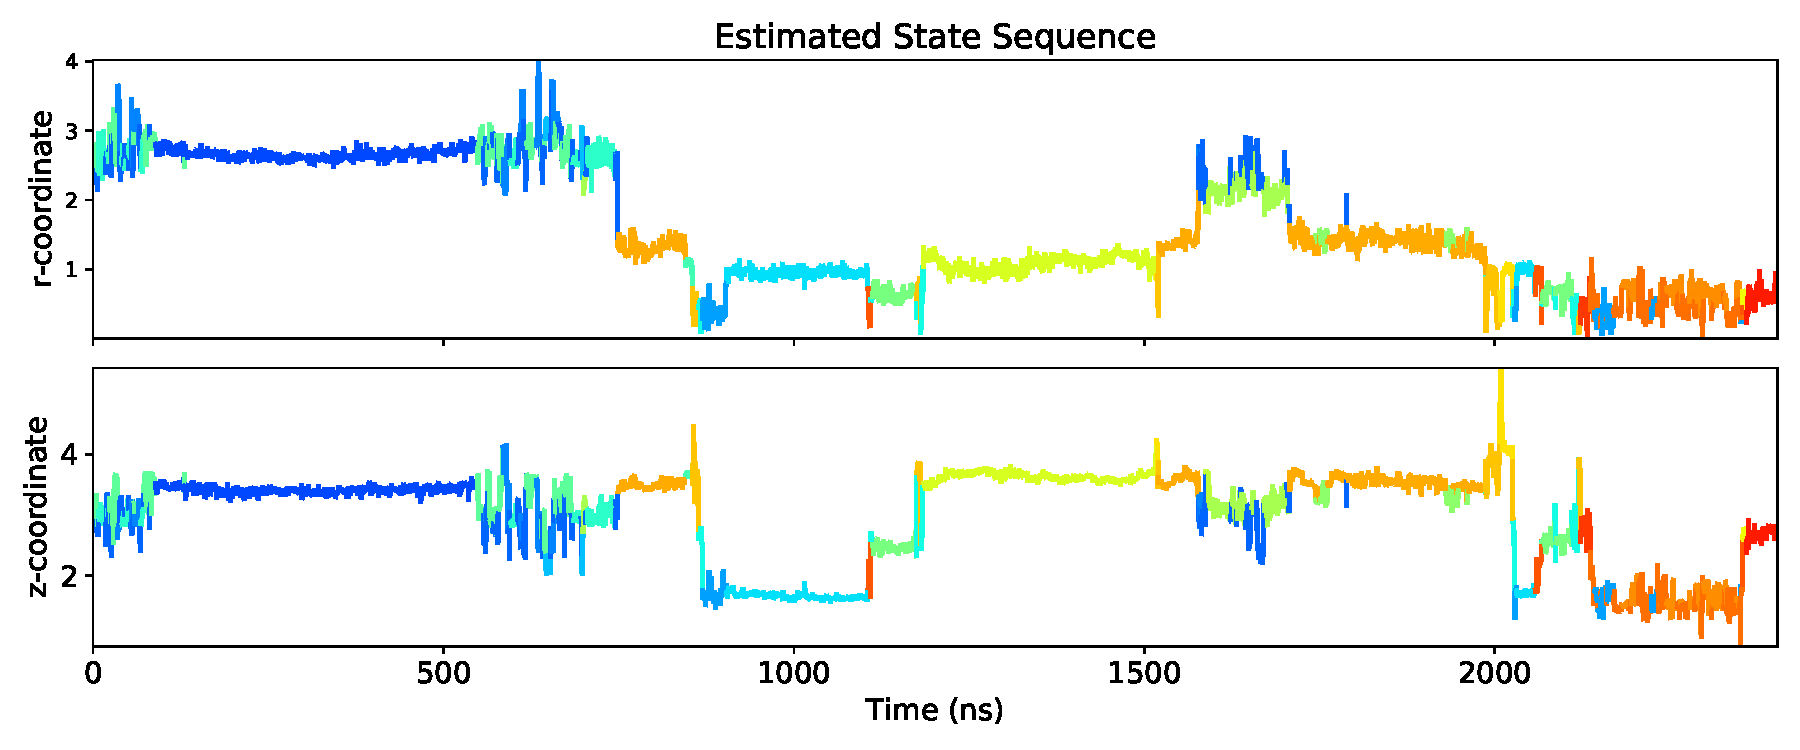
\includegraphics[width=\textwidth]{rz_unclustered_MET.pdf}
  \caption{The HDP-AR-HMM found 24 distinct VAR(1) states in this representative methanol trajectory.
  We performed the parameterization in 3D Cartesian coordinates, but for this figure, we 
  converted to cylindrical coordinates, with $r$ the distance from the pore center, to 
  provide a clearer picture of solute motion.}\label{fig:rz_unclustered}
  \end{figure}
  
  \subsection{Reproducing MD Trajectories and MSDs with the HDP-AR-HMM}\label{section:unclustered_MSD_prediction}

  Before analyzing solute behavior characteristic to the states identified by the
  HDP-AR-HMM, it is important to verify whether the state dynamics are consistent with MD
  both qualitatively and quantitatively. Therefore, we generated stochastic 
  realizations based on the parameters of each trajectory as described in 
  Section~\ref{method:realizations}.
  
  As shown in Figure~\ref{fig:qualitative_unclustered}, realizations of our model 
  can produce trajectories that show qualitatively similar hopping and trapping 
  behavior to the MD trajectories to which they were fit. It is important that our
  model reproduces this behavior so that we can have confidence in its usefulness
  for quantitative predictions.
  
  % BJC4: This figure needs to be redone with new trajectory generation procedure
  \begin{figure}
  \centering
  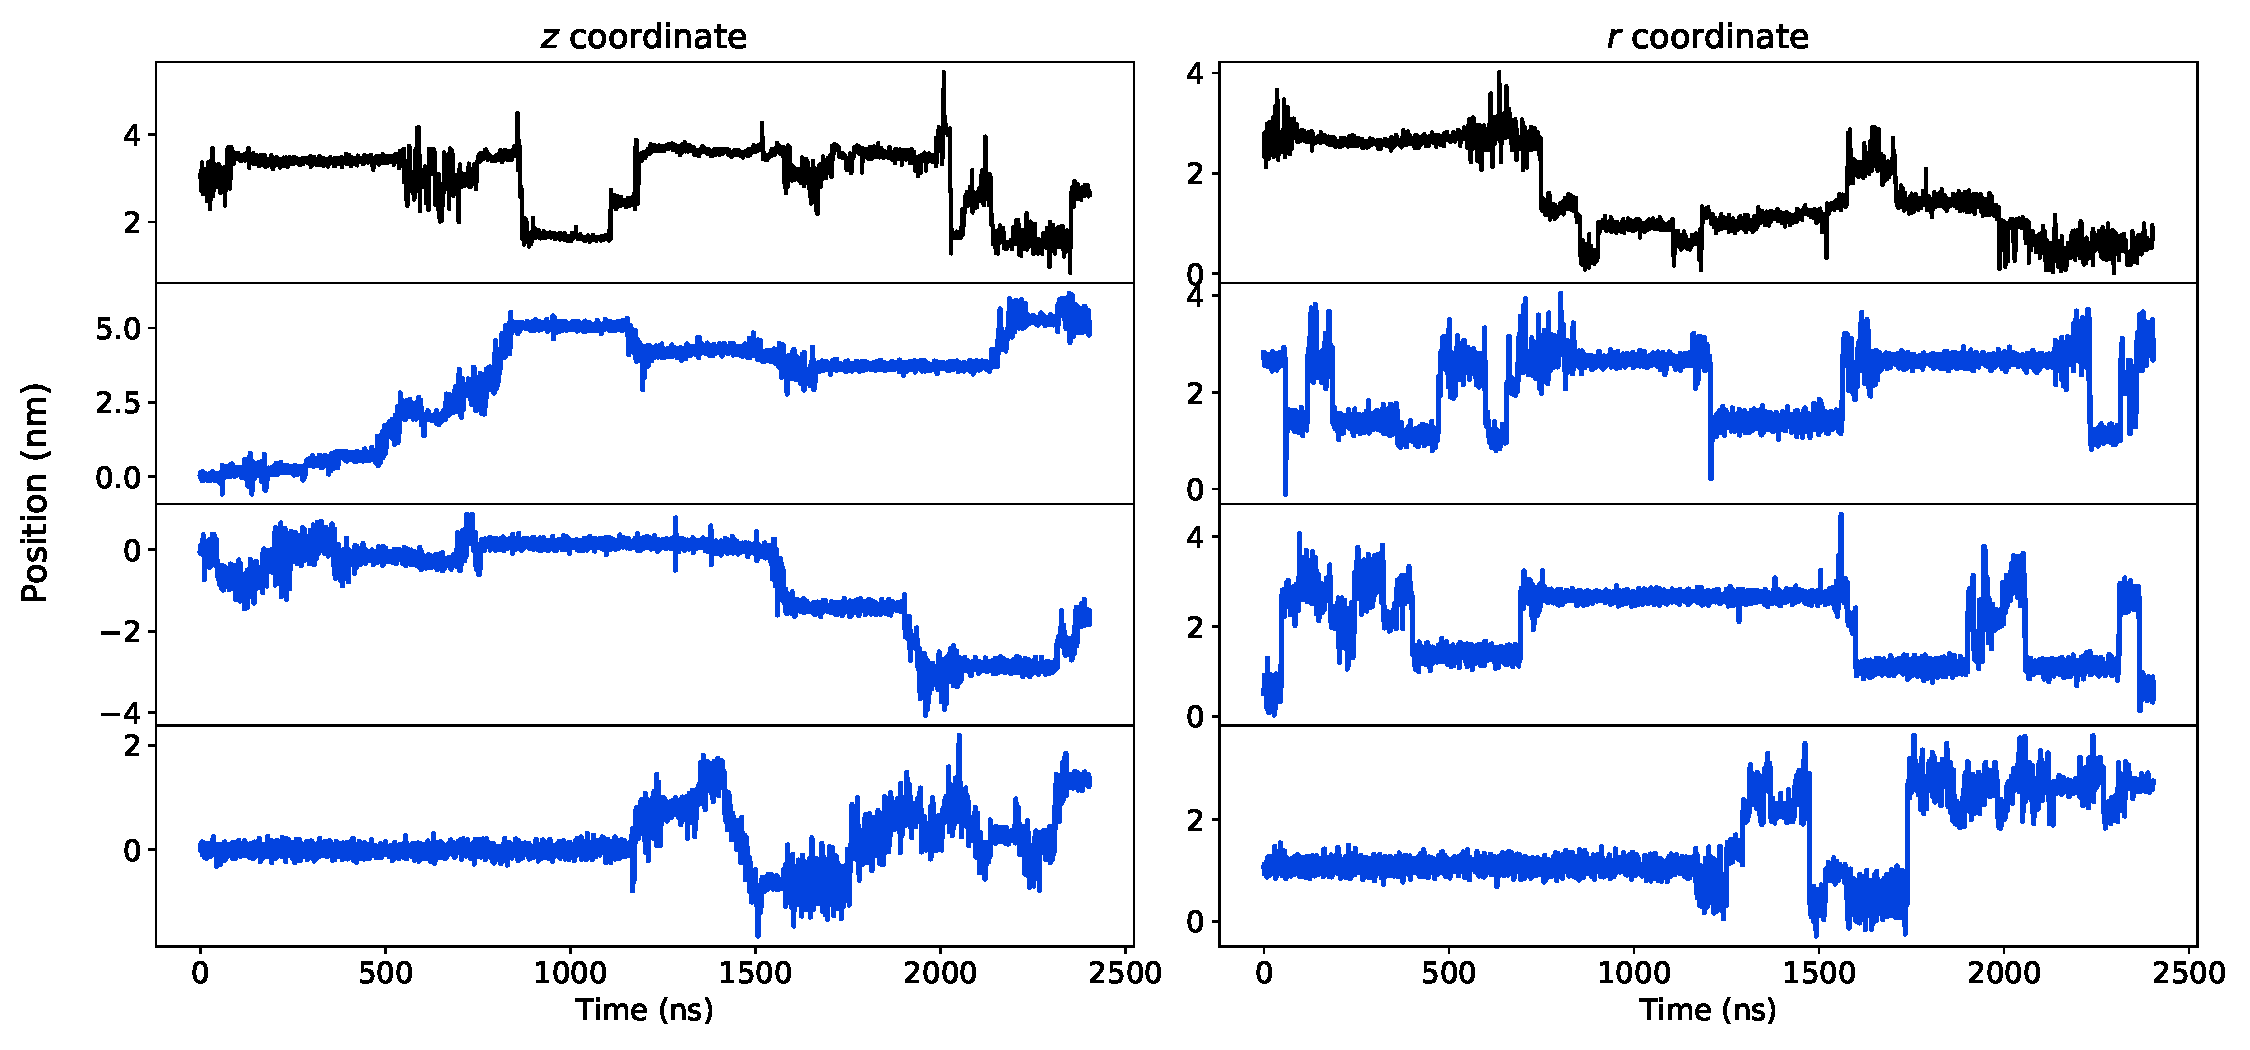
\includegraphics[width=\textwidth]{qualitative_unclustered_MET2.pdf}
  \caption{We can use realizations of the HDP-AR-HMM to generate trajectories which 
  bear qualitative resemblance to the MD trajectories. We used the parameters 
  of the HDP-AR-HMM, whose state segments are visualized in 
  Figure~\ref{fig:rz_unclustered}, in order to construct an ensemble of 
  characteristic trajectories. Solute trajectories generated with
  the HDP-AR-HMM (blue) show the same hopping and trapping behavior exhibited by 
  MD (black).
  }\label{fig:qualitative_unclustered}
  \end{figure}
  
  In Figure~\ref{fig:unclustered_msds}, we show that in most cases we can reproduce the 
  MD MSDs on long timescales within uncertainty using realizations of the 
  HDP-AR-HMM.
  \begin{itemize}
    \item We generated the MSD curves using Method 1 described in 
    Section~\ref{method:realizations} of the methods.
    \item Our ability to reproduce these curves gives use confidence
    in their long term predictions.
    \item We underestimate the MSD of urea because of a small number of MD 
    trajectories with uncharacteristically high MSDs. Despite our best efforts, 
    we could not adequately parameterize an HDP-AR-HMM which reproduced said 
    behavior. (see SI)  %BJC4: TODO
    \item On long timescales, the model appear to have the same slope as 
    the MD trajectory.
  \end{itemize}
  
  \begin{figure}
  \centering
  \begin{subfigure}{0.24\textwidth}
  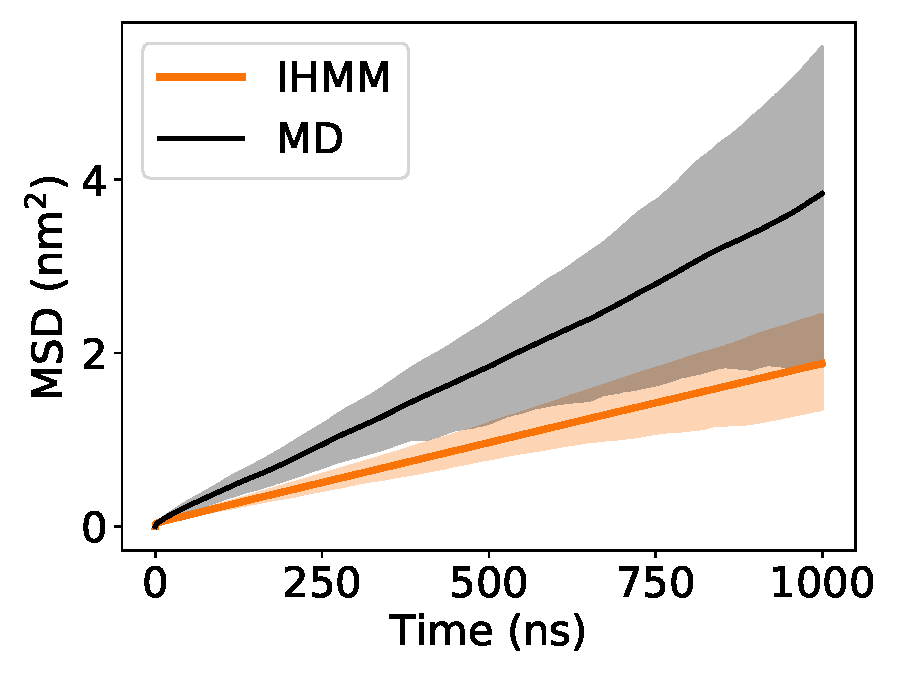
\includegraphics[width=\textwidth]{unclustered_msd_MET.pdf}
  \caption{methanol}\label{fig:unclustered_msd_MET}
  \end{subfigure}
  \begin{subfigure}{0.24\textwidth}
  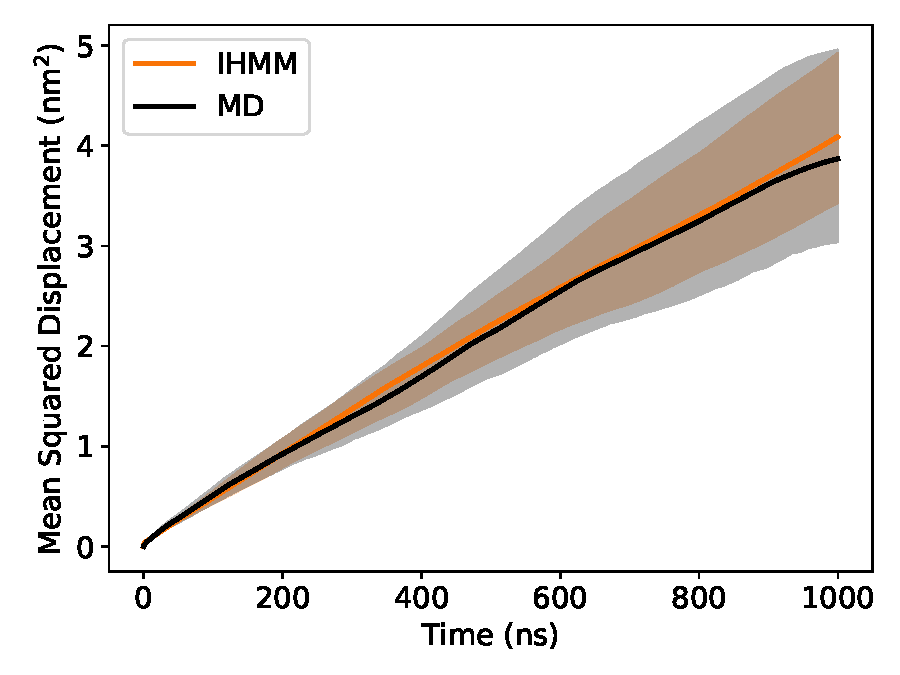
\includegraphics[width=\textwidth]{unclustered_msd_GCL.pdf}
  \caption{ethylene glycol}\label{fig:unclustered_msd_GCL}
  \end{subfigure}
  \begin{subfigure}{0.24\textwidth}
  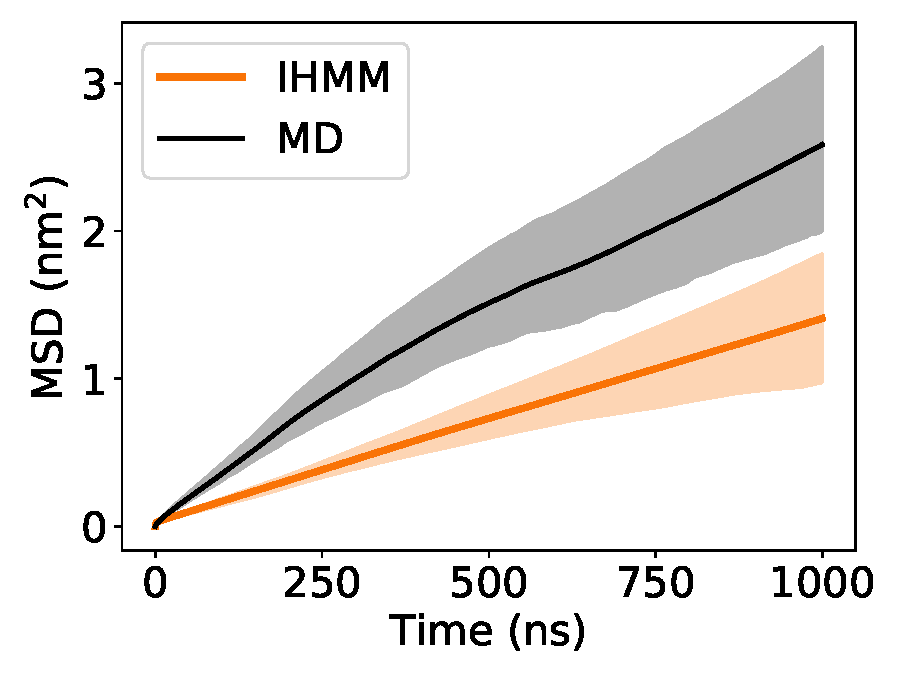
\includegraphics[width=\textwidth]{unclustered_msd_URE.pdf}
  \caption{urea}\label{fig:unclustered_msd_URE}
  \end{subfigure}
  \begin{subfigure}{0.24\textwidth}
  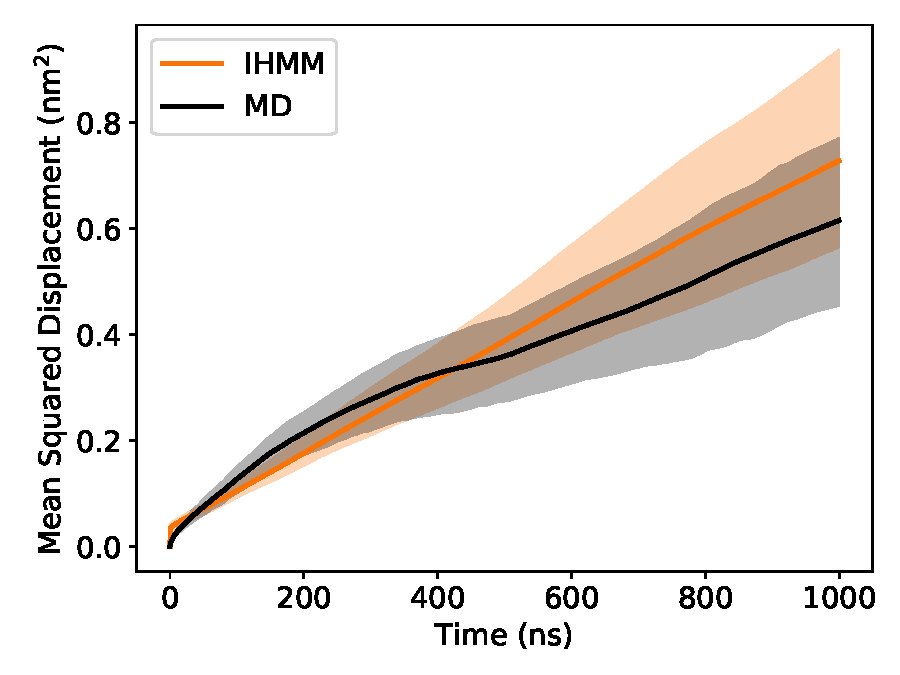
\includegraphics[width=\textwidth]{unclustered_msd_ACH.pdf}
  \caption{acetic acid}\label{fig:unclustered_msd_ACH}
  \end{subfigure}
  \caption{The MD MSDs (black) of methanol and urea are under-predicted by 
  the HDP-AR-HMM (orange), while the predictions match within uncertainty for ethylene
  glycol and acetic acid}\label{fig:unclustered_msds}
  \end{figure}
  
  \subsection{Using HDP-AR-HMM Parameters to Predict Selectivity}\label{section:macroscopic_properties}
  
  Since we can generate trajectories that share features similar to MD simulations, 
  it is now reasonable to project solute behavior onto much longer time scales.
  \begin{itemize}
    \item The HDP-AR-HMM MSD predictions quickly enter a linear regime, therefore we can 
    project long timescale MSDs based on the predicted diffusion constant as described
    in Section~\ref{method:selectivity}.
  \end{itemize}  
  
  % BJC4: figure here
  
  % BJC4: some kind of brief selectivity analysis here. This easy, I'll get that done 
  % tonight or tomorrow.
  
  \subsection{Learning Mechanisms from the HDP-AR-HMM}\label{section:mechanisms}
  
  Solutes in this system show a wide range of behavior influenced by the 
  heterogeneity of the membrane's nanostructure as well as the interactions 
  between monomer and solute chemical functionality. Our application of the 
  HDP-AR-HMM can identify and distinguish these behaviors. The following approach 
  to analysis demonstrates how one can discover and explain the very complex
  behavior exhibited by solutes over long MD trajectories in terms of 
  solute-membrane interactions.
  
  \textit{State Clustering}: In order to reduce the state space to a more 
  manageable size, and to allow different solute trajectories to share 
  similar behavior, we clustered the states identified by the HDP-AR-HMM for each
  solute as described in Section~\ref{method:clustering}. In 
  Figure~\ref{fig:clustered_traj_MET}, we show the results of clustering on the 
  same methanol trajectory from Figure~\ref{fig:rz_unclustered}. Based on 
  the criteria described in Section~\ref{method:clustering},
  we chose to reducing the total state space for methanol from 287 to \nclusters. 
  
  Our goal is to derive the simplest model which adequately distinguishes
  different types of solute motion. By working to understand the parameters of 
  each cluster, we can uncover the associated transport mechanisms responsible
  for those parameters.
  
  \begin{figure}
  \centering
  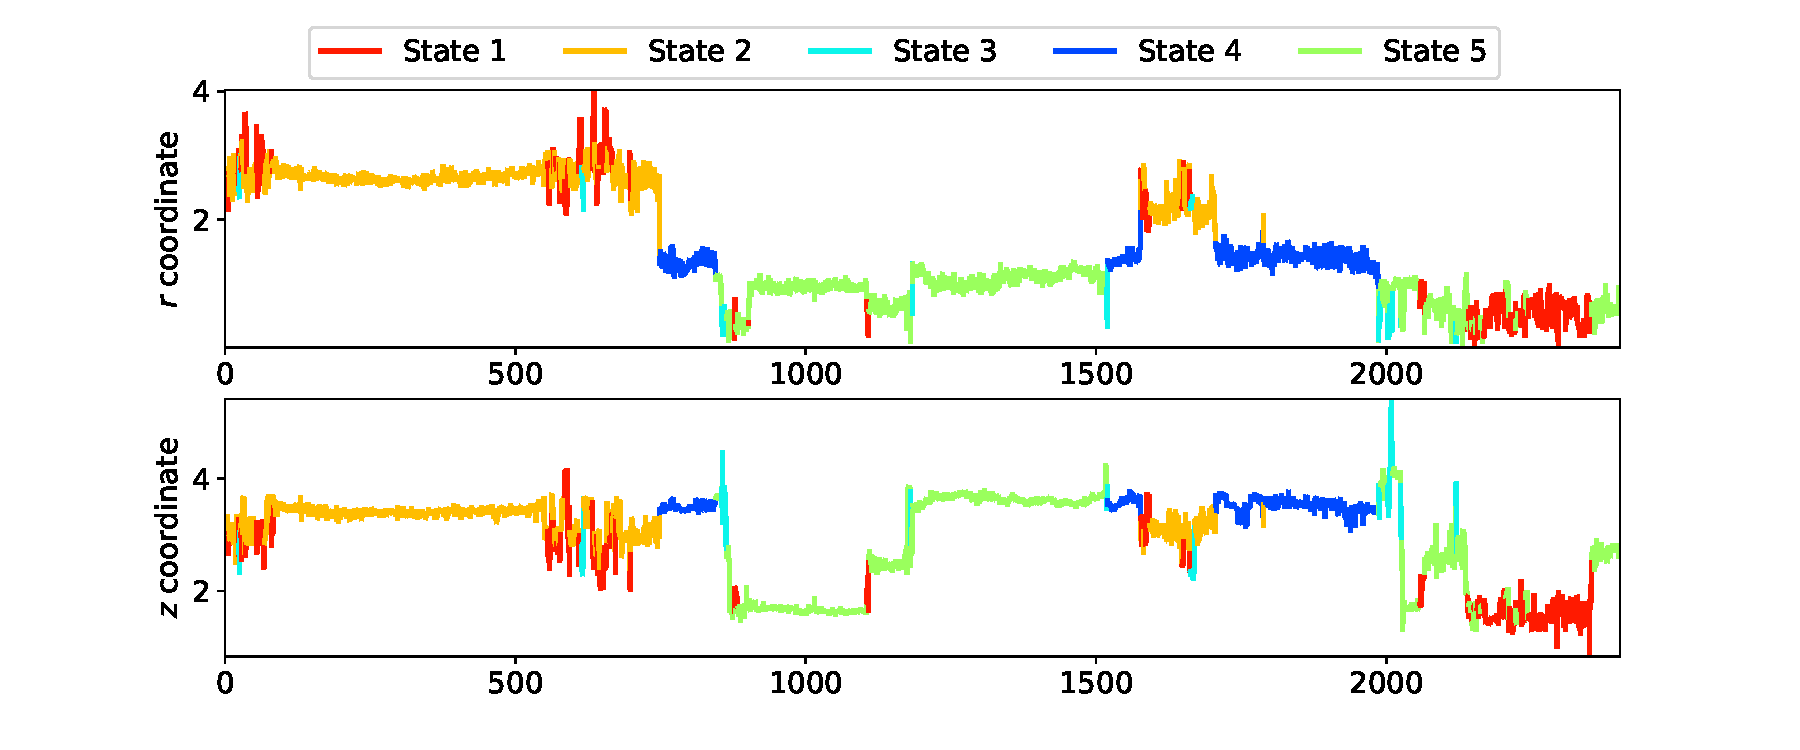
\includegraphics[width=\textwidth]{clustered_traj_MET_ward_10.pdf}
  \caption{We reduced the total state space from 287 to 10 total states 
  shared across all trajectories. For the trajectory in this figure, we reduced
  the total number of states from 24 (see Figure~\ref{fig:rz_unclustered}) to
  5.}\label{fig:clustered_traj_MET}
  \end{figure}
  
  \textit{Dynamics of clustered parameter sets}: The clustered parameter sets
  allow transitions between dynamics exhibited by the same solute from independent 
  trajectories. This allows us to create hybrid trajectories which draw on all
  solute behavior.
  
  Realizations based on the 10 clustered parameter sets do not show the same
  qualitative dynamics as the MD simulation trajectories. 
  \begin{itemize}  
    \item In Figure~\ref{fig:qualitative_clustered_MET}, we compare MD 
    trajectories to realizations of our model using the clustered parameter sets.
    \item They lack the diversity of behavior which we see in the MD simulation trajectories.
    \item They do not show the same range of trapping times and hop lengths.
    \item If we use a higher number of clusters, the qualitative match improves, but
    at the cost of a larger state space to interpret (see Figure~\ref{S-fig:qualitative_improvement}
    of the Supporting Information).
  \end{itemize}
  
  In addition to qualitative mismatches, realizations of the clustered HDP-AR-HMM 
  under-predict the unclustered MSD predictions and the MD MSD. 
  \begin{itemize}
    \item Much of a solute's MSD is likely a consequence of short-lived trapping states
    with high variances.
    \item When clustering, disjoint segments with similar enough parameters are
    re-parameterized together as part of the same state, lengthening the lifetimes 
    of very short-lived states and suppressing the fluctuations of high variance states.
    \item In Figure~\ref{fig:clustered_MSD}, it is evident that increasing the number
    of clusters increases the predicted MSD.
    \item Matching the unclustered MSDs would likely require many more clusters, at 
    which point the benefits of clustering are lost. 
    %BJC: I don't think the following discussion is necessary anymore.
%    \item In Figure~\ref{fig:dwell_distributions}, we compare the overall dwell time
%    distributions generated directly from MD simulations to that generated from 
%    realizations of the HDP-AR-HMM. 
%    \item We do this by measuring the time spent in each independent same-state segment.
%    \item Some of the probability density of short trapping times in the MD simulations 
%    gets shifted to medium length trapping times in realizations of the HDP-AR-HMM. 
%    \item In Figure~\ref{fig:dwell_distributions_modT} and~\ref{fig:msd_modT}, we show 
%    that by modifying the transition matrix to encourage transitions towards states with
%    shorter dwell times, we can more closely reproduce the dwell time distribution and 
%    MSD of MD. This is because most solute motion is a consequence of transitions between
%    trapped states.
  \end{itemize}
  
  \begin{figure}
  \centering
  \begin{subfigure}{0.63\textwidth}
  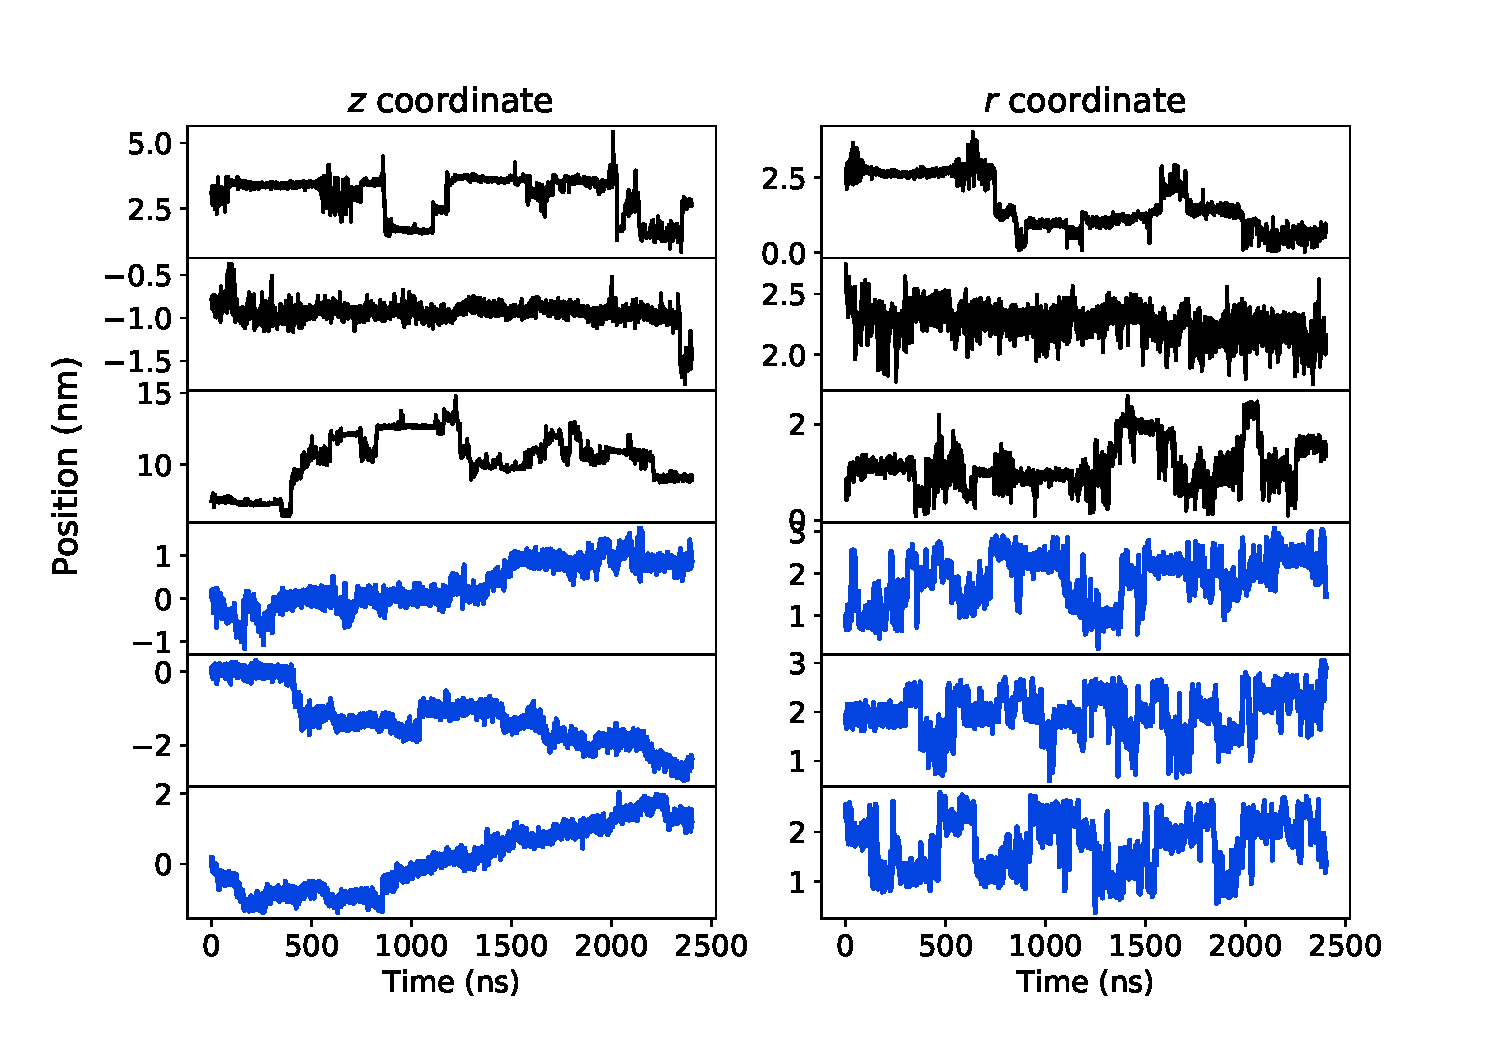
\includegraphics[width=\textwidth]{qualitative_clustered_MET_10.pdf}
  \caption{}\label{fig:qualitative_clustered_MET}
  \end{subfigure}
  \begin{subfigure}{0.35\textwidth}
  \vspace{2.25em}
  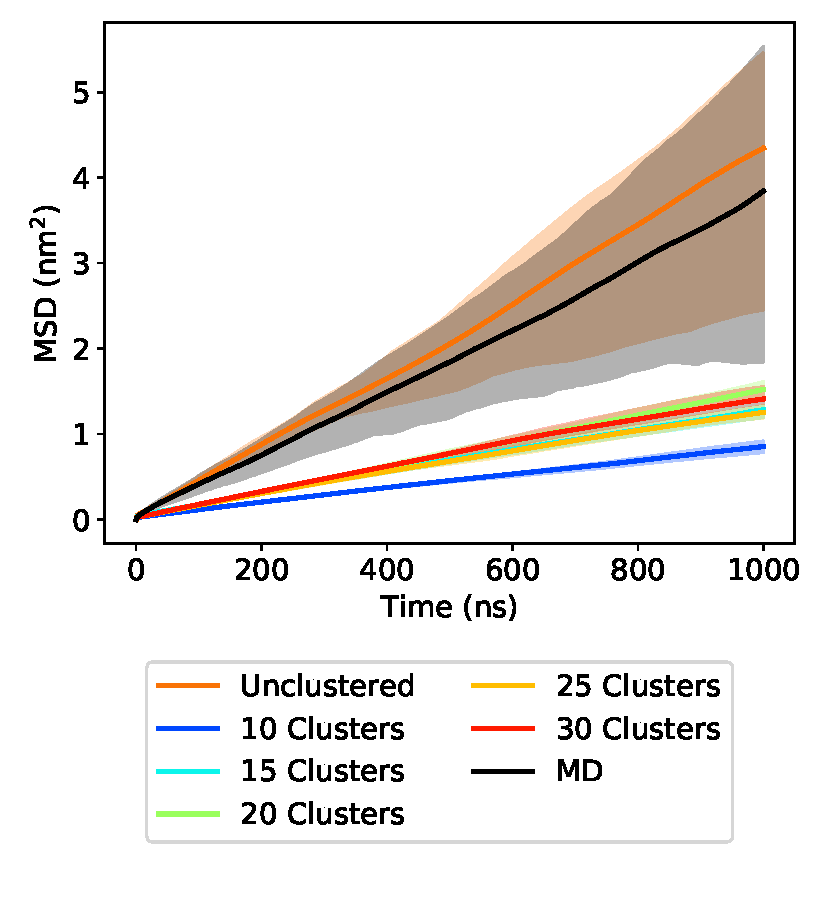
\includegraphics[width=\textwidth]{msd_nclusters.pdf}
  \caption{}\label{fig:clustered_MSD}
  \end{subfigure}
  \caption{(a) Stochastic trajectory realizations generated from our model (blue) based on
  the clustered methanol parameters do not qualitatively reproduce the diversity of behavior
  seen in our MD trajectories. (b) MSD predictions by clustered parameter sets consistently
  under-predict MD MSD. They appear to do a better job of predicting MSDs as the number
  of clusters increases.}\label{fig:clustered_dynamics}
  \end{figure}
  
  \textit{The dynamics of frequently occurring states}: We may learn the most by 
  studying the dynamical modes common to the majority of the solute trajectories.
  \begin{itemize}
  	\item Of the 10 state clusters, only 5 appear in a significant number of 
  	solute trajectories (Figure~\ref{fig:prevalence}).
  	\item Although a majority of the solutes visit these 5 dominant states the
  	amount of time spent in each varies widely. 
  \end{itemize} 
  
  \begin{figure}
  \centering
  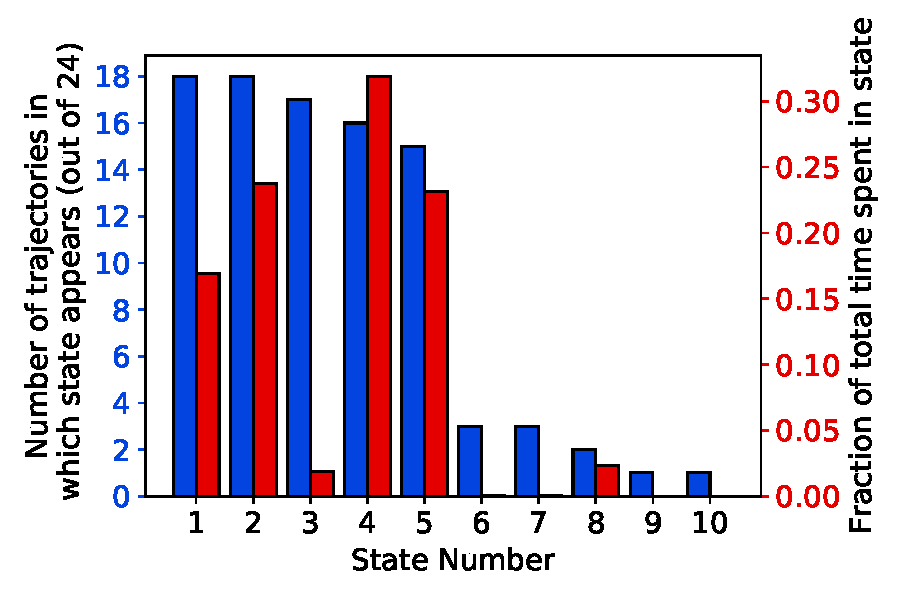
\includegraphics[width=0.5\textwidth]{prevalence.pdf}
  \caption{5 out of the 10 clustered states are visited by 15 or more of the solute
  trajectories. The solutes spend varying amounts of time in each of these states.
  }
  \label{fig:prevalence}
  \end{figure}
  
  We can begin to hypothesize mechanisms by studying the behaviors defined by the 
  state parameters.
  \begin{itemize}
  	\item In Figure~\ref{fig:common_states_lines}, we plot representative 
  	dynamics of each of the five most visited states.
  	\item The states exhibit a range of autoregressive and trapping behavior
  	throughout the membrane pores.
%  	\item There is good representation by states across a range of radial distances
%  	from the pore centers. 
  \end{itemize}
  
  Since the radial means are weighted averages of the states used to parameterize
  each cluster, for interpretive purposes, it is important to recognize that the means
  only provide clues towards the general location of the solute. 
  \begin{itemize}
  	\item For example, the radial mean of state 3 is 1.4 nm from the pore center. 
  	\item However, inspection of Figure~\ref{fig:clustered_traj_MET} suggests that this 
  	type of behavior actually occurs radially throughout the pore.
  	\item There are instances of state 3 less than 1 nm from the pore center and more 
  	than 2 nm from the pore center. 
  	\item In this case, the radial mean only suggests that this type of behavior 
  	happens in both regions somewhat equally.
  \end{itemize}
  
  Solutes exhibit a range of autoregressive behavior as shown by the representative 
  solute trajectories in Figure~\ref{fig:common_states_lines} and the scatter
  plot in Figure~\ref{fig:A_sigma_scatter}.
  \begin{itemize}
  	\item In most cases, the eigenvalues of $A$ and $\Sigma$ appear nearly paired
  	in their radial and axial dimensions, which implies nearly symmetric behavior 
  	with off-diagonals both matrices near zero.
  	\item The most notable exception is state 3, which has a much higher radial 
  	eigenvalue of the covariance matrix.
  	\item Both eigenvalues of state 3's covariance are actually quite
  	large. This implies relatively large fluctuations in the $z$ direction and even
  	bigger fluctuations in the $r$ direction.
  	\item All states have slightly lower covariance in the axial direction. It's
  	likely easier for solutes to move laterally rather than to move up through the
  	alkane chains.
  	\item States 3 and 4 show a strong previous-hop dependence (high $A$) while
  	the rest of the states have a somewhat weaker dependence.
  \end{itemize}

  Solutes are trapped for various lengths of time.
  \begin{itemize}
    \item On average, state 4 has the longest dwell times and state 3 has
    the shortest dwell times while the rest have intermediate dwell times.
    \item This is somewhat supported by inspection of Figure~\ref{fig:clustered_traj_MET},
    however. 
	\item The expected dwell times of the clusters incorporate all 24 trajectories.
%    \item Once again, since we clustered, it is important to avoid studying
%    the exact dwell time values, and to focus on their relative magnitudes.
  \end{itemize}
  
  % BJC4: Not sure if this is useful.
  By studying the parameters, it is now easier to describe the state behavior.
  \begin{enumerate}[label={State \theenumi :}, leftmargin=3.5\parindent]
     \item This state has intermediate dwell times with high past-hop dependence.
     The radial mean and evidence from Figure~\ref{fig:clustered_traj_MET} suggests
     that this state is common in the tail and pore region.
     \item This state seems to occur exclusively in the tail region based on its radial
     mean. Its fluctuations are small and there is little past hop dependence
     \item This is likely a hopping state that strongly contribute to the solute's MSD. 
     It is short lived and takes very large hops. This type of behavior is exhibited 
     near and far from the pore center as discussed earlier.
     \item This is a trapping state with a strong dependence on its previous fluctuation.
     Evidence from Figure~\ref{fig:clustered_traj_MET} and a radial mean of 1.8 suggest
     that it tends to occur at intermediate distances from the pore center.
     \item This is an intermediate-length trapping state that occurs close to the pore
     center. It's fluctuations are tight and relatively independent of its previous 
     fluctuation.
  \end{enumerate}
  
  \begin{figure}
  \centering
  \begin{subfigure}{0.58\textwidth}
  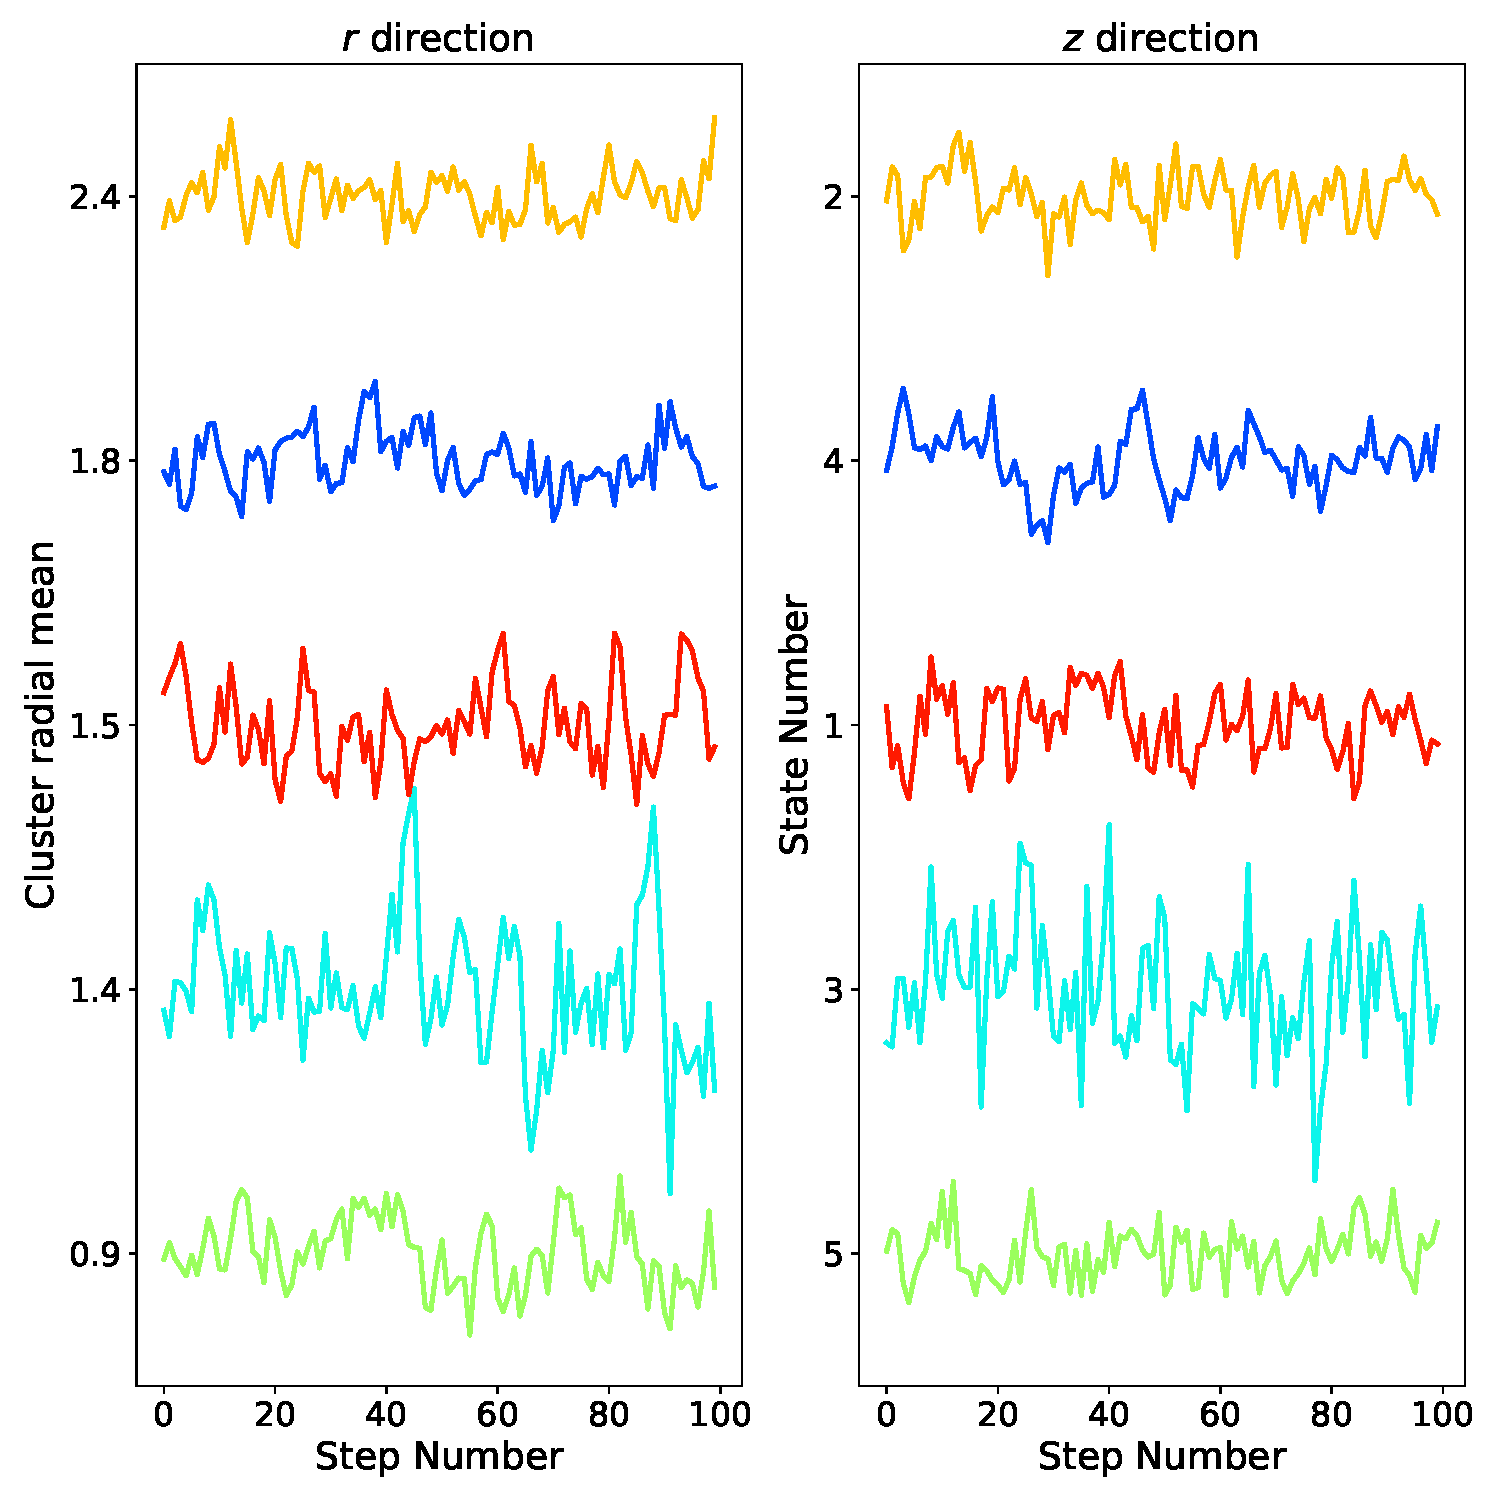
\includegraphics[width=\textwidth]{common_states.pdf}
  \caption{}\label{fig:common_states_lines}
  \end{subfigure}
  \begin{subfigure}{0.41\textwidth}
  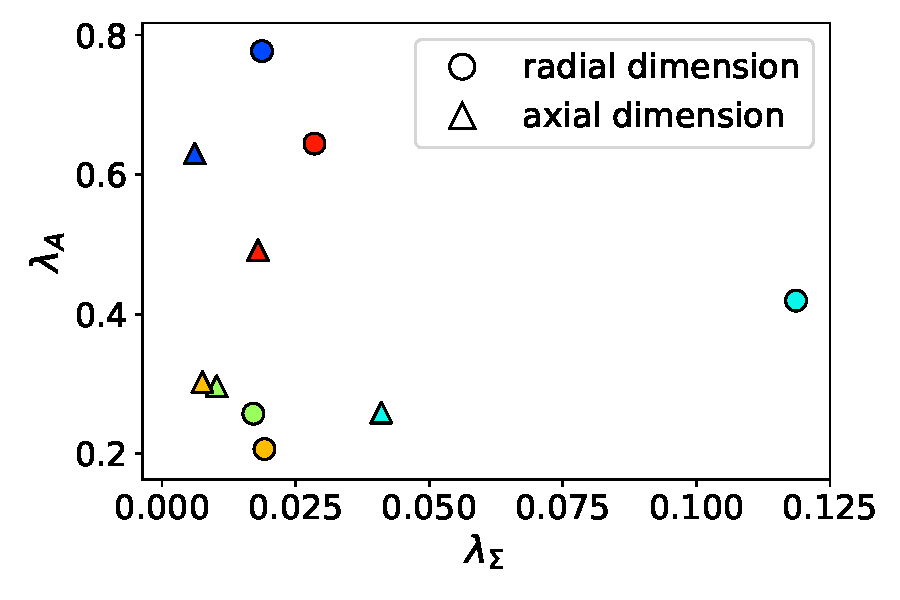
\includegraphics[width=\textwidth]{A_sigma_scatter.pdf}
  \caption{}\label{fig:A_sigma_scatter}
  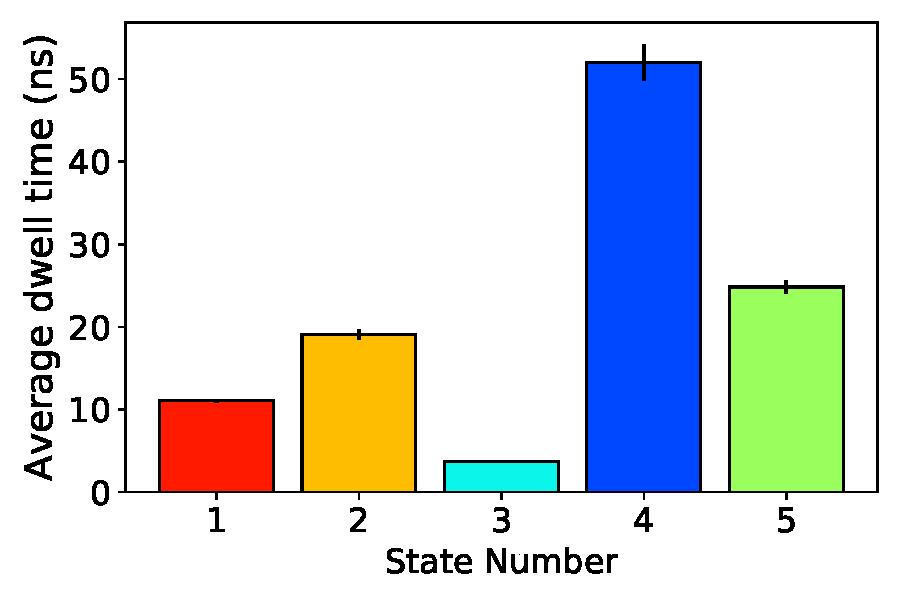
\includegraphics[width=\textwidth]{dwell_times.pdf}
  \caption{}\label{fig:dwell_times}
  \end{subfigure}
  \caption{The 5 most visited states by methanol show a range of dynamical behavior. In 
  (a), we show representative dynamics of these states. All time series have a mean of zero and are
  shifted to put the mean in line with the $y$-axis labels for the purpose of visualizing them.
  The $y$-axis labels of the $r$ coordinate plot specify the radial mean of each clustered 
  state. All of the states pictured appear in the trajectory shown in 
  Figure~\ref{fig:clustered_traj_MET} and are colored to match.
  (b) We can begin to understand the solute behaviors demonstrated in (a) by understanding their VAR 
  parameters. Higher values of $\lambda_{\Sigma}$ generally are indicative of large fluctuations
  and higher values of $\lambda_A$ indicate strong previous-hop dependence of the fluctuations.
  (c) Using Equation~\ref{eqn:dwell_times}, we estimated the expected time spent within each 
  of the states.
  }\label{fig:common_states_MET}
  \end{figure}
   
  \textit{Relating Parameters to Solute-Membrane Interactions}: Based on the
  molecules and ions which constitute the membrane, it is straightforward to 
  hypothesize two types interactions that might occur.
  \begin{itemize}  
    \item All of the solutes are polar and have hydrogen bond donating and 
    accepting groups. 
    \item The monomers have 10 oxygen atoms distributed from head to tail that are 
    capable of accepting hydrogen bonds. 
    \item Also, the ionic bond between the head groups and sodium ions can
    be easily broken since both components can be stabilized by surrounding 
    water molecules and solutes.
    \item Therefore, it is logical to search for hydrogen bonding interactions
    and solute association with sodium ions.
  \end{itemize}
  
  For methanol, hydrogen bonding is a much more dominant interaction than sodium
  ion association. 
  \begin{itemize}
    \item In Figure~\ref{fig:hbond_fractions}, we show that methanol participates
    in hydrogen bonds to various parts of the monomer between 27 and 45\% of the
    total time it occupies the dominant states.
    \item Methanol associates with sodium ions less than 10\% of the time in 
    dominant states.
  \end{itemize}  
  
  The distribution of types of hydrogen bonds and associated hydrogen bond lifetimes
  varies by dominant state.
  \begin{itemize}
    \item States 1 and 2 are dominated by hydrogen bonds to the head groups and, to 
    a smaller extent, the ether linkages.
    \item State 1 methanol molecules that donate hydrogen bonds to the tail oxygen 
    atoms exhibit by far the longest hydrogen bond lifetimes among all states.
    \item States 3 and 4 hydrogen bond to all regions of the monomer relatively 
    evenly, which is consistent with our earlier observation that states 3 and 4
    are representative of behavior seen radially throughout the membrane pores.
    \item State 3 has the lowest hydrogen bond and sodium association lifetimes 
    which is consistent with its short dwell times. These are fleeting interactions
    since it is likely a jumping state.
    \item Methanol molecules in state 5 hydrogen bond almost exclusively to the 
    carboxylate head groups and ether linkages which is consistent with the radial
    mean of the cluster.
  \end{itemize}
  
  \begin{figure}
  \centering
  \begin{subfigure}{0.475\textwidth}
  \centering
  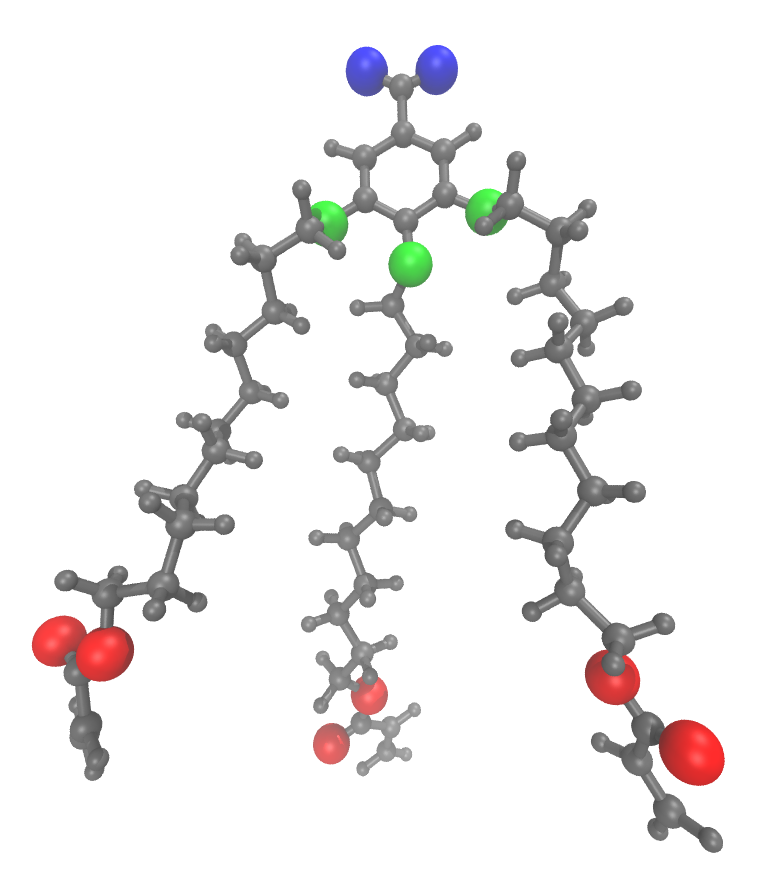
\includegraphics[width=0.6\textwidth, angle=0]{monomer_oxygens.png}
  \caption{}\label{fig:monomer_oxygens}
  \end{subfigure}
  \begin{subfigure}{0.475\textwidth}
  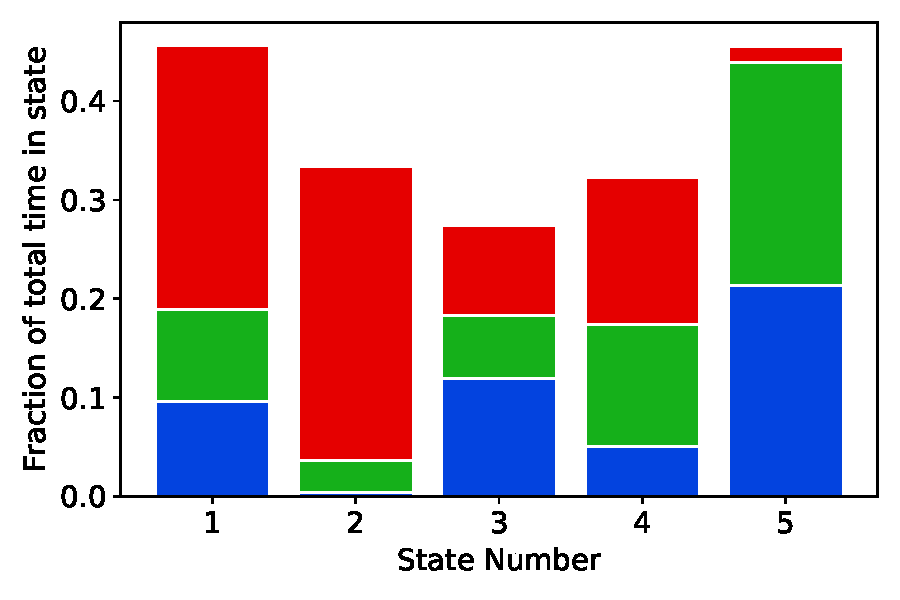
\includegraphics[width=\textwidth]{hbond_fractions.pdf}
  \caption{}\label{fig:hbond_fractions}
  \end{subfigure}
  \begin{subfigure}{0.475\textwidth}
  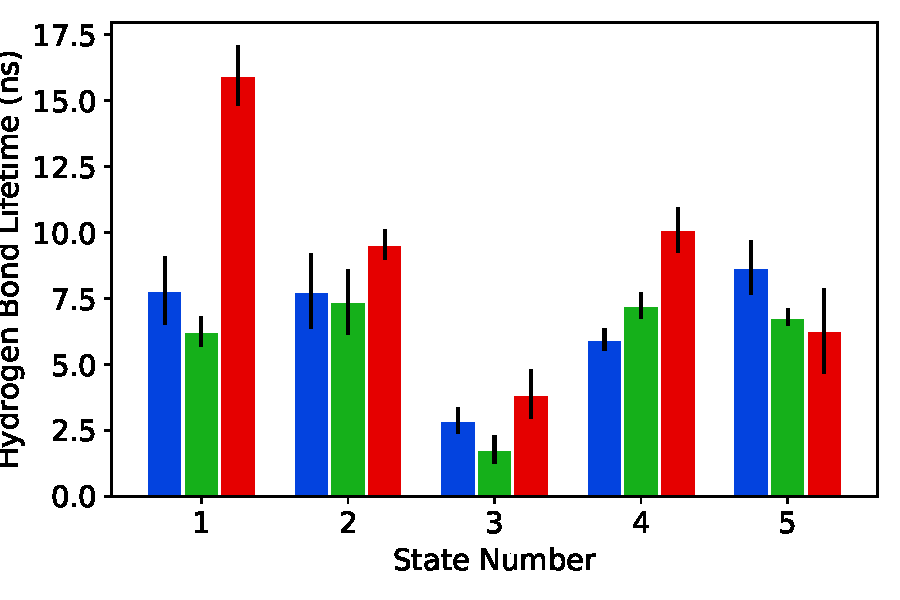
\includegraphics[width=\textwidth]{hbond_lifetimes.pdf}
  \caption{}\label{fig:hbond_lifetimes}
  \end{subfigure}
  % BJC4: I put this one here for compact-ness. Not sure if I should separate into own figure
  \begin{subfigure}{0.475\textwidth}
  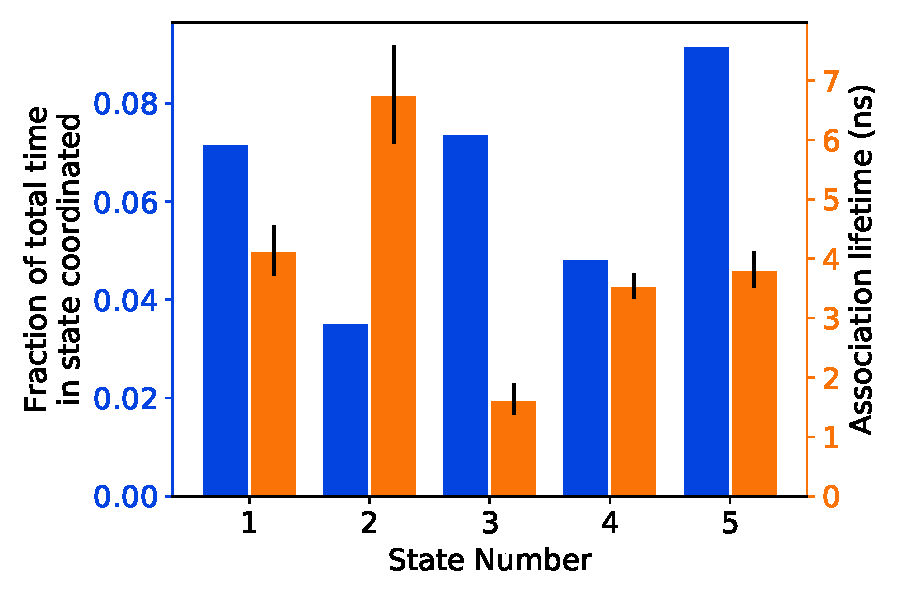
\includegraphics[width=\textwidth]{association_fraction_lifetimes.pdf}
  \caption{}\label{fig:association_fraction_lifetimes}
  \end{subfigure}
  \caption{(a) We analyzed hydrogen bond donation to the highlighted oxygen atoms in three 
  regions of the monomer: the carboxylate groups (blue), the ether linkages (green) and the
  tails (red). (b) For each dominant state, we plotted the fraction of the total time in
  that state spent hydrogen bonding to various regions of the monomer, color coded to match (a).
  (c) For each type of hydrogen bond in each dominant state, we calculated the 95th percentile
  of hydrogen bond lifetimes. (d) We also analyzed the frequency and lifetimes of solute 
  association with sodium ions. Methanol associates with sodium less than 10\% of the total 
  time it occupies any of the dominant state.
  %Relative to hydrogen bonding, it is a relatively infrequent interaction
  %for methanol molecules, but the 
  }
  \label{fig:hydrogen_bonding}
  \end{figure}
  
  The local number density of heavy atoms surrounding solutes help round out methanol's
  mechanistic picture.
  \begin{itemize}
    \item Although hydrogen bonding interactions are relatively frequent, methanol molecules
    are unbound by any measurable electrostatic interactions about half or more of the 
    simulation time.  
    \item Figure~\ref{fig:local_densities} helps to illustrate how the local density of 
    membrane components can aid in solute entrapment.
    \item When solutes experience long trapping times, the local number density of heavy 
    atoms is larger.
    \item Even when hydrogen bonds break, surrounding alkane density likely helps keep
    the solutes in place allowing them to eventually reform. This can happen deep in the
    tails or close to the monomer head groups.
    \item Methanol molecules which experience State 3 have by far the smallest local 
    number density which is likely responsible for their mobility, as suggested by the state's
    large covariance.
  \end{itemize}
  
  \begin{figure}
  \centering
  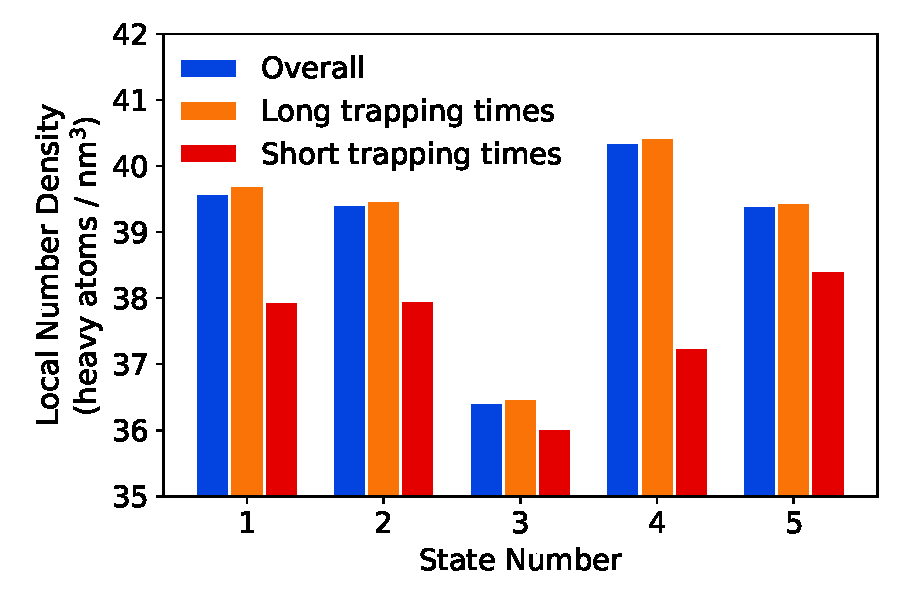
\includegraphics[width=0.5\textwidth]{local_densities.pdf}
  \caption{We measured the local number density of heavy atoms surrounding solutes in each
  state. In blue, we plot the local number density experienced by solutes averaged over all
  frames in which the solute occupied the given state. We broke down this overall average 
  number density into number densities measured from instances when the state is occupied 
  for long (orange) versus short(red) dwell time states. We define define `long' dwells times
  as the 50th percentile of all dwell times in the given state, and short as all others. It
  is clear that solutes which experience longer dwells times are also surrounded by more 
  heavy atoms on average.}\label{fig:local_densities}
  \end{figure}
  
  \subsubsection*{Comparison of Solute Behavior}
  
  We can apply a similar analysis to the other solutes in this study. We can likely
  learn new information through comparison of solute behavior with metrics based on
  the chemical intuition gained by studying methanol.
  
  The size and chemical functionality of the solutes dictates the interactions which
  influence solute transport.
  \begin{itemize}
    \item In Figure~\ref{fig:hbonds_assoc_summary}, we show that the solutes donate
    hydrogen bonds and associate with sodium ions to varying degrees.
    \item In fact methanol, by far, interacts the least by these mechanisms.
    \item This is likely because methanol is very small and it is easier for it to partition
    into the tail region where there are fewer groups with which it can interact (see
    Figure~\ref{fig:rdf_summary}).
    \item Acetic acid, urea and ethylene glycol are slightly larger than methanol
    and contain multiple polar substituents which stabilize them closer to the 
    pore region.
    \item These three solutes also participate in significantly more sodium ion
    association. 
    \item In our previous work, we showed that the sodium ions frequently associate
    with the carbonyl groups of acetic acid and urea.
  \end{itemize}
  
  \begin{figure}
  \centering
  \begin{subfigure}{0.325\textwidth}
  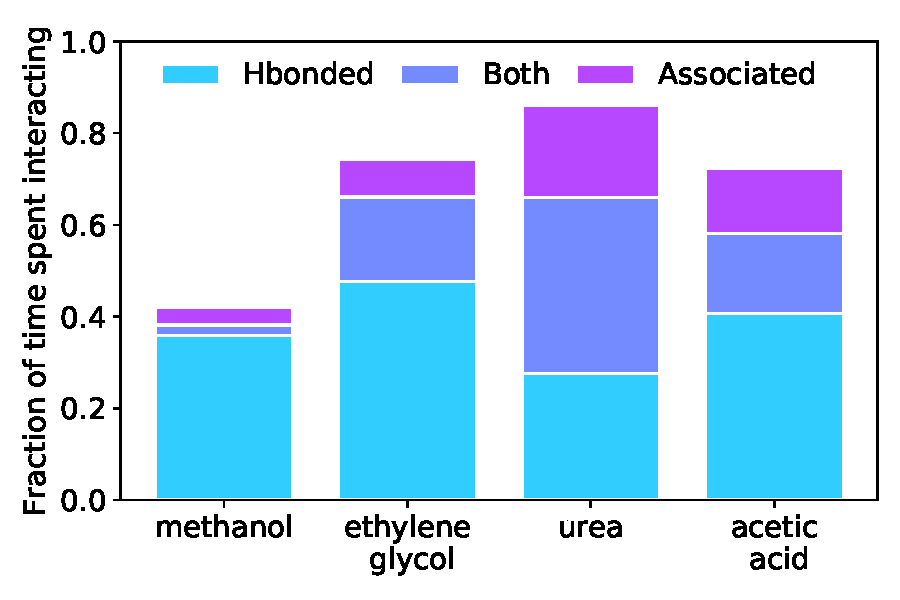
\includegraphics[width=\textwidth]{hbonds_assoc_summary.pdf}
  \caption{}\label{fig:hbonds_assoc_summary}
  \end{subfigure}
  \begin{subfigure}{0.325\textwidth}
  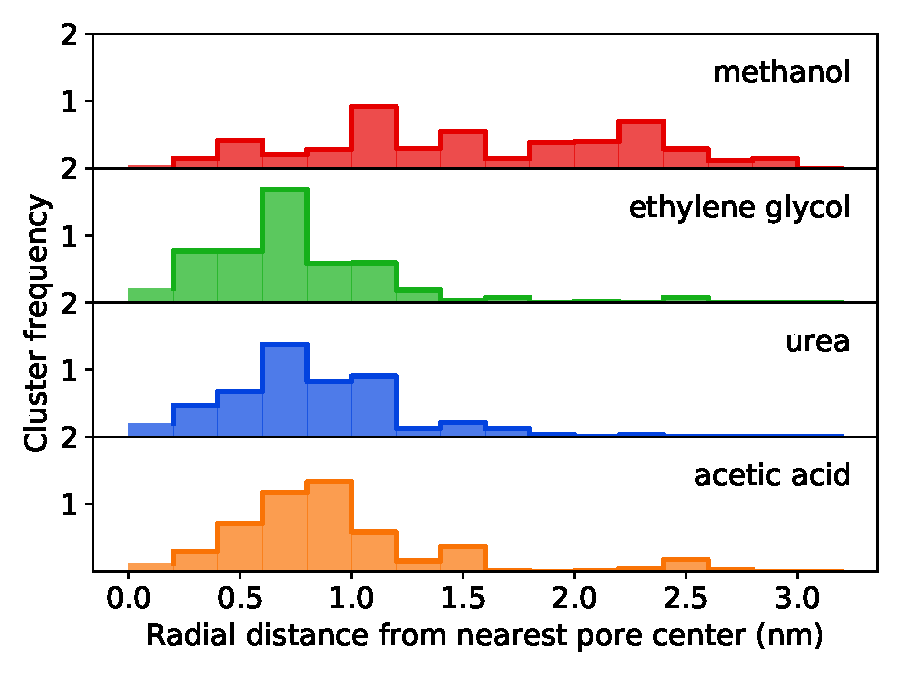
\includegraphics[width=\textwidth]{rdf_summary.pdf}
  \caption{}\label{fig:rdf_summary}
  \end{subfigure}
  \begin{subfigure}{0.325\textwidth}
  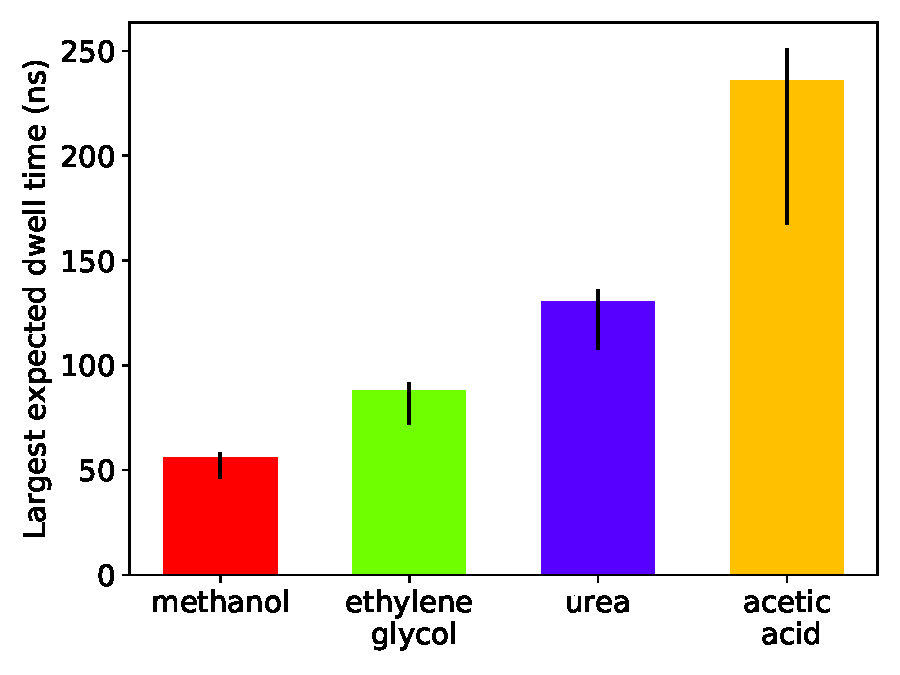
\includegraphics[width=\textwidth]{dwell_time_summary.pdf}
  \caption{}\label{fig:dwell_time_summary}
  \end{subfigure}
  \caption{(a) Solutes hydrogen bond and associate with sodium ions
  to different degrees. Sometimes, they participate in both interactions at
  once. (b) We histogrammed the radial means of the unclustered states weighted
  by the length of time spent in that state. Most solutes spend the majority of
  their time close to the pore center. Only methanol has a significant density
  far from the pore center. (c) The largest expected dwell time among the dominant 
  clustered states for each solute are inversely related to the solute's MSD. 
  }\label{fig:summaries}
  \end{figure}
  
  Solutes with dominant clusters characterized by long dwell times tend to 
  have lower MSDs.
  \begin{itemize}
    \item In Figure~\ref{fig:dwell_time_summary}, we plot the expected dwell
    time of each solute in the dominant state which has the the highest
    self-transition probability. 
    \item The trend in MSDs is inversely related to the trend in maximum
    expected dwell times.
    \item Both acetic acid and urea participate in many hydrogen bonds and
    sodium ion association interactions and the states visited by both solutes
    have similar distributions of radial means, however acetic acid is 
    subject to much longer dwell times, and hence a lower MSD.
    % BJC4: I could dig further into this. Not sure if worth it.
    \item This may be because acetic acid is a stronger hydrogen bond donor
    than urea. 
    \item Could also be that the urea is still mobile while paired with sodium ions.
  \end{itemize}
  
  \section{Conclusion}
  
  We have shown that the HDP-AR-HMM can be used to automatically parameterize solute 
  time series with an unknown number of latent dynamical modes. Initially, we applied
  the algorithm to each trajectory independently. Using the model parameters fit
  to each trajectory, we generated stochastic realizations of solute trajectories that
  can qualitatively and quantitatively reproduce the behavior of MD solute 
  trajectories. The realizations show the hopping and trapping behavior that is
  characteristic of polar solutes in this system. 
  
  By pooling MSDs predicted by models fit to each trajectory, we can reproduce
  the solute MSDs measured directly from the our MD-simulated trajectories. 
  The low computational expense of generating these stochastic trajectories allows
  one to project solute behavior on much longer timescales, allowing us to predict
  selectivity, an experimentally-relevant quantity.
  
  In order to gain a mechanistic understanding of solute motion, we showed how 
  we could cluster the parameter sets in order to reduce the state space down
  to an interpretable size. We coupled analysis of the clustered parameter sets
  with measurements of membrane properties and solute-membrane interactions 
  in order to gain a detailed understanding of the diverse sets behavior 
  exhibited by solutes in these membranes. We showed how
  solute motion is influenced by hydrogen bonding, sodium ion association and local
  membrane density.
  
  When clustering, our goal was to create the simplest model possible that gave
  clear mechanistic insight. This is important for systems where transport mechanisms
  are not easily hypothesized. However, once one gains some mechanistic understanding,
  as we have in this work, the clustering procedure can be modified in order to 
  study specific interactions or radially dependent behavior.
  
  Although we showcase this modeling approach by example, but it is important to
  recognize the generality of this analysis, especially in the context of molecular
  simulations. Vector autogregressive models can describe a diverse set of behavior
  and so the HDP-AR-HMM may be suited to study many types motion, including those not 
  characterized by hopping and trapping. The HDP-AR-HMM is a powerful approach for 
  understanding particle motion as well as for generating inexpensive models
  which can give macroscopic insight.
  
  \section*{Supporting Information}

  Detailed explanations and expansions upon the results and procedures mentioned in
  the main text are described in the Supporting Information. 
  %This information is
  %available free of charge via the Internet at http://pubs.acs.org.

  \section*{Acknowledgments}

  This work was supported in part by the ACS Petroleum Research Fund
  grant \#59814-ND7 and the Graduate Assistance in Areas of National Need (GAANN) 
  fellowship which is funded by the U.S. Department of Education. 
  Molecular simulations were performed using the Extreme Science and
  Engineering Discovery Environment (XSEDE), which is supported by National
  Science Foundation grant number ACI-1548562. Specifically, it used the Bridges
  system, which is supported by NSF award number ACI-1445606, at the Pittsburgh
  Supercomputing Center (PSC). This work also utilized the RMACC Summit supercomputer,
  which is supported by the National Science Foundation (awards ACI-1532235 and
  ACI-1532236), the University of Colorado Boulder, and Colorado State
  University. The Summit supercomputer is a joint effort of the University of
  Colorado Boulder and Colorado State University.

  \clearpage

  \bibliographystyle{ieeetr}
  \bibliography{hdphmm}

  %\newpage

  %\section*{TOC Graphic}

\end{document}

% LocalWords:  BJC micropollutants Desalination permeability nanofiltration LLC
% LocalWords:  Amphiphilic nanostructures Lyotropic amphiphilic lyotropic MSDDM
% LocalWords:  solutes selectivities solute nanoscopic timescales MSDs MSD HMMs
% LocalWords:  nonparameteric Parrinello Rahman barostat rescale transitioning
% LocalWords:  al's HMM Dirichlet HDP DP Wishart TODO SI al MATLAB teh gael pdf
% LocalWords:  nonparametric bayesian solute's reparameterized intracluster ca
% LocalWords:  delocalize Luzar Chandler histogrammed interpolator methanol's
% LocalWords:  nanostructure carboxylate VMD nonidealities hbonds outlier GAANN
% LocalWords:  autogregressive PRF ACS XSEDE ACI HDP-AR-HMM nanoporous flowback evy
% LocalWords:  timescale subdiffusive coscia subdiffusion calderon GROMACS der
% LocalWords:  berendsen gromacs spoel hess emailed plateauing hmm ne gelman AR
% LocalWords:  walt numpy GCL URE ACH IMMM subsubsection modT convective vmd Na
% LocalWords:  scannable subsubcaptions errorbars uncharacteristicness facelift
% LocalWords:  PSC RMACC hdphmm TOC nominalizations dischinger ramaseshan Baum
% LocalWords:  functionalized teuerle jasra markov bioinformatics hughes yoon
% LocalWords:  hines diarization MJLSs MJLS SLDSs SLDS hamada jk params MNIW
% LocalWords:  plateaued nclusters leftmargin trans diffusivity sorption alkane
% LocalWords:  ness substituents
